\documentclass[12pt, letterpaper]{article}
\usepackage{graphicx}
\usepackage{hyperref}
\usepackage{amssymb}
\usepackage{amsmath}
\usepackage{float}
\usepackage{mathtools}
\usepackage{enumitem}
\usepackage[margin=1in]{geometry}
\usepackage[figurename=Figura]{caption}

\title{%
  Situación Problema: Análisis de Audio usando Fourier \\
  \large F1009: Análisis de métodos matemáticos para la física}
\author{}

\begin{document}

\maketitle

\begin{tabular}{ccc}
Juan Pablo Guerrero Escudero & Romina Nájera Fuentes & Juan Braulio Olivares Rodríguez\\
ITESM, Querétaro & ITESM, Querétaro & ITESM, Querétaro\\
A01706810@tec.mx & A01424411@tec.mx & A01706880@tec.mx
\end{tabular}


\section{Introducción}
En los últimos años, se han hecho populares aplicaciones y programas de reconocimiento de 
canciones a partir de un fragmento de ellas, y aunque estos algoritmos son patentados, varios de ellos
utilizan los principios del análisis espectral, utilizando Análisis de Fourier. Este análisis
resulta una herramienta muy útil para esto, ya que, por medio de la Transformada de Fourier, provee frecuencias de 
la canción, y el uso de espectogramas permite sacar conclusiones de este sonido. Por medio de 
este concepto matemático, se puede analizar el fenómeno físico de las ondas de audio, que son ondas longitudinales 
en un medio (principalmente aire) que el ser humano es capaz de escuchar a distintas frecuencias. En este reporte, se 
hará una investigación sobre los conceptos físicos y matemáticos necesarios, y se analizarán 10 canciones, para 
tratar de identificar el género de cada una, entre música instrumental y reggaetón, demostrando así una de las múltiples aplicaciones reales de las matemáticas en la física.
\section{Teoría}

\subsection{Conceptos físicos}

\subsubsection{Ondas de sonido}
De acuerdo a Young y Freedman \cite{university-physics}, el sonido se define como una onda 
longitudinal en un medio, principalmente aire, pero pueden ser otros como gases, líquidos o sólidos. Las 
ondas de sonido más simples son ondas sinusoidales con una frecuencia, amplitud y longitud definida. 
\cite{university-physics}. El ser humano es capaz de escuchar ondas en el rango de 20 a 20,000 Hz, con 
frecuencias por encima del rango (ultrasónicas) o debajo del rango (infrasónicas) de escucha humano. 
De acuerdo a Hwaitat \cite{frequencies-wave-sound-pso}, las ondas de sonido son peturbancias propagadas por un medio que 
no se ve afectado, y éstas ondas pueden ser ya sea longitudinales, o transversales. Para una onda 
de tipo longitudinal, el medio vibra en ángulos rectos al movimiento de la onda, y en el caso de ondas longitudinales, 
el medio vibra en la misma dirección que el movimiento.En la Figura \ref*{Ondas Longitudinales} se observa gráficamente lo discutido. 
\begin{figure}[H]
  \centering
  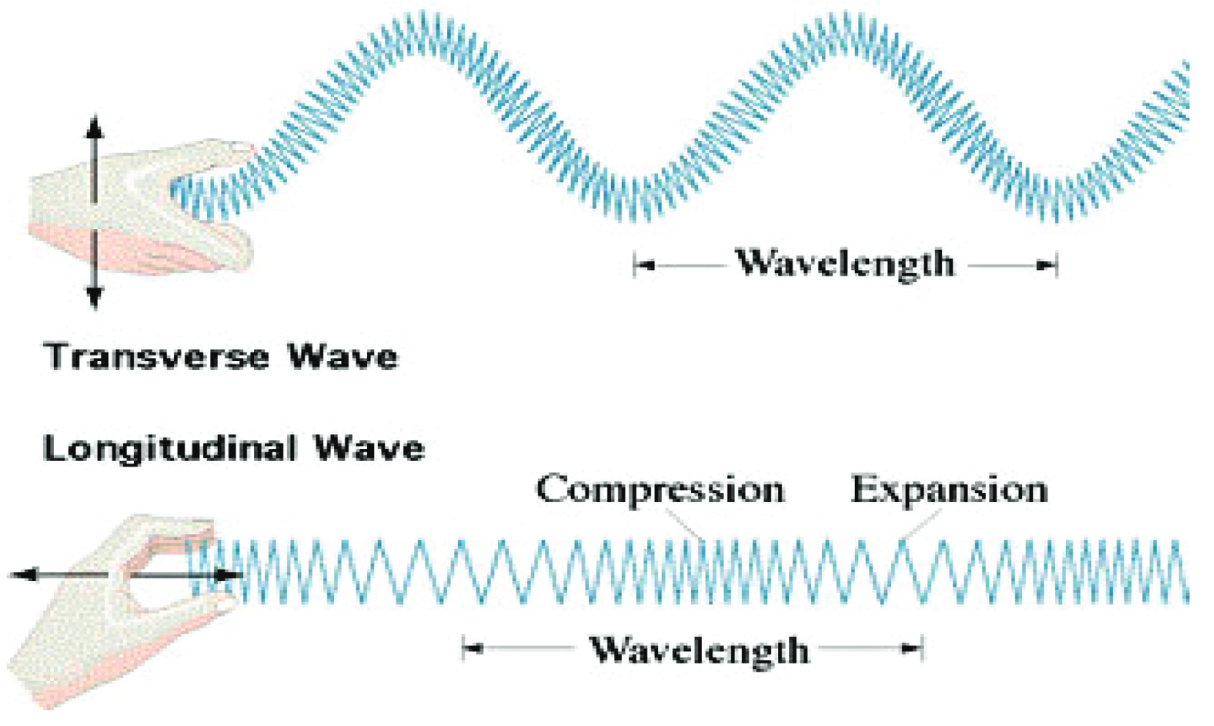
\includegraphics[height = 4cm]{imgs/investigacion/ondas_longitudinales_transversales.png}
  \caption{Ondas longitudinales y transversales}
  \label{Ondas Longitudinales}
\end{figure}
Los parámetros de cualquier onda constituyen la amplitud, la frecuencia 
y la longitud, mencionados anteriormente. La amplitud puede ser definida como la "altura" 
de la onda, la frecuencia se define como los ciclos por segundo, y la longitud se define como la distancia 
entre un pico de onda y otro. Para una vista gráfica, vea la Figura \ref*{parametros-ondas}. Generalmente, sucede que 
cuando dos partículas están en movimiento en el mismo medio, ocurre interferencia. Ésto significa que 
las amplitudes de onda son sumadas algebráicamente, y se siguen moviendo por el medio sin distracciones. En el mundo real, 
la interferencia de ondas crea patrones complejos, y puede ser muy difícil de analizar.  
\begin{figure}[H]
  \centering
  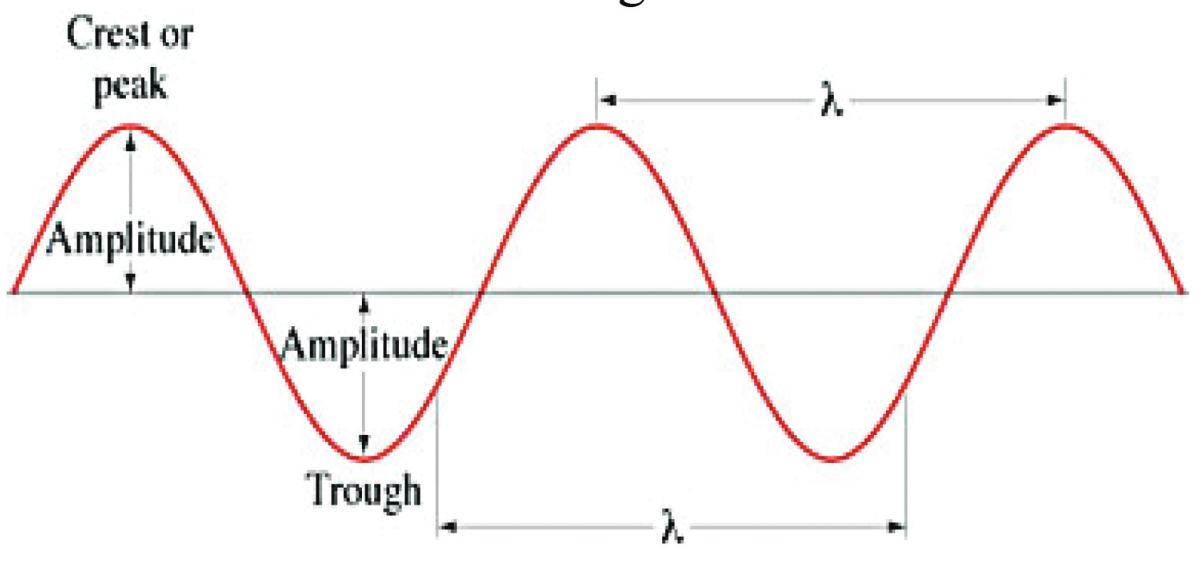
\includegraphics[height = 4cm]{imgs/investigacion/parametros-ondas.png}
  \caption{Parámetros de las ondas de sonido}
  \label{parametros-ondas}
\end{figure}
\subsubsection{Frecuencias de audio/sonido}
Como se definió anteriormente, la frecuencia de una onda es, de acuerdo a \cite{university-physics}, como el número de repeticiones 
    de una función periódica durante una unidad de variación en la variable independiente. En otras palabras, es el número de 
    ocurrencias de un evento repetitivo por unidad de tiempo. Matemáticamente, se dice que en medios no dispersivos (medios donde 
    la velocidad de la onda es independiente de la frecuencia), la frecuencia tiene una relación inversa con la longitud 
    de onda, en la forma de la ecuación \ref{frequency-eq}, donde $\lambda$ es la longitud de la onda, y $v$ es la velocidad de la onda.
    \begin{align}
    f = \frac{v}{\lambda}
    \label{frequency-eq}
    \end{align}Analizando la ecuación \ref{frequency-eq}, observamos que ondas de longitud más corta ($\lambda$), 
    tienen mayores variaciones en la frecuencia debido a que los máximos y mínimos están más cerca uno del otro, y viceversa. Una vista gráfica 
    se observa en la Figura \ref{frecuencias-onda}. 
    \begin{figure}[H]
      \centering
      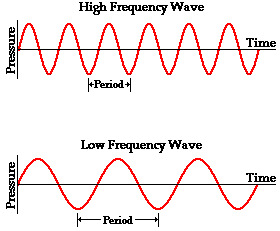
\includegraphics[height = 6cm]{imgs/investigacion/frecuencias-ondas.jpg}
      \caption{Diferentes frecuencias de onda}
      \label{frecuencias-onda}
    \end{figure}
    Además, la frecuencia se mide en Hz o Hertz, equivalente a un evento de repetición por segundo. De acuerdo a \cite{university-physics}, 
    la frecuencia de una onda de sonido es el factor primario al determinar el tono de un sonido. Frecuencias 
    más altas emiten sonidos con mayor tono que frecuencias más bajas. En conjunto, cuando se juntan diferentes frecuencias 
    al mismo tiempo, se crean patrones más complejos que ondas simples sinusoidales, debido a que físicamente, las variaciones en presión 
    del medio que se generan son más complejas. 

\subsubsection{Sonidos armónicos}

De acuerdo a \cite{university-physics}, puede suceder que dos tonos producidos por diferentes instrumentos tengan la 
misma frecuencia pero suenen diferente, y ésto es debido a la diferencia en contenido armónico, que está definido como la colección de diferentes frecuencias 
que componen un sonido complejo formado por muchas frecuencias fundamentales. Además, de acuerdo a \cite{university-physics}, otro factor que determina los 
sonidos armónicos de un sonido es el comportamiento al inicio (attack) y al final (decay) de cada tono. Cada instrumento posee una diferente dinámica de sonidos armónicos, 
lo cuál entrega ondas en una mezcla de frecuencias diferentes, que da su sonido característico. \\

Para dar algunos ejemplos \cite{orchestra-frecuency}, la nota de afinación en una orquesta sinfónica es A4, que tiene una frecuencia de 440Hz. Frecuencias más complejas se generan cuando 
se utiliza el concepto de octavas en música, que de acuerdo a \cite{octave-definition}, es una serie de 8 notas musicales que ocupan el intervalo entre 2 notas, una teniendo el doble 
o la mitad de la frecuencia que la otra. Es decir, un salto de una octava corresponde a duplicar la frecuencia de la onda de sonido. 
\subsubsection{Beats}
En la física, sucede que cuando se tienen dos ondas con igual amplitud pero ligeramente diferentes frecuencias, si ambas ondas van hacia la 
misma dirección, pasa que en ciertos momentos, las dos ondas están en la misma fase, es decir, sus máximos coinciden y sus amplitudes se suman. Sin embargo, 
debido a que las ondas están en ligeramente distintas frecuencias, llega a haber momentos en los que estas ondas están 
exactamente fuera de fase, y se cancelan una con otra. La variación de amplitud causa variaciones en el volumen, llamadas \textit{beats}, y la frecuencia 
con la que éstos varían se le llama frecuencia de beat. En la Figura \ref{beats-grafica} se muestra éste proceso de manera gráfica.
\begin{figure}[H]
  \centering
  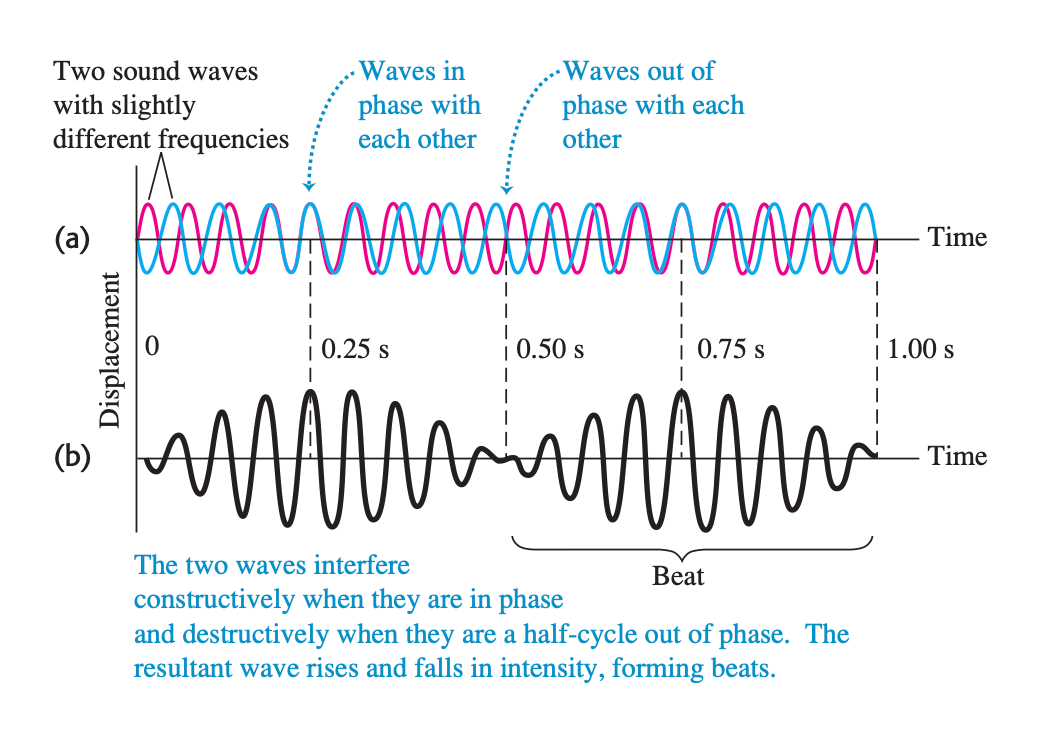
\includegraphics[height = 7cm]{imgs/investigacion/beats-grafica.png}
  \caption{Gráfica del proceso de beats}
  \label{beats-grafica}
\end{figure}Los beats entre dos tonos, de acuerdo a \cite{university-physics}, pueden ser escuchados hasta una frecuencia de beat de 6 o 7Hz. En la práctica, 
una técnica importante es escuchar los beats para afinar los instrumentos musicales. Además, de acuerdo a \cite{university-physics}, cuando las diferencias de 
frecuencia son mayores a 7Hz, se dejan de escuchar beats individuales, y las frecuencias se mezclan en una de consonancia o disonancia, dependiendo de la 
naturaleza de las frecuencias. 
\subsection{Análisis de las canciones}

Para la clasificación de las canciones entre los géneros de música instrumental o reggaetón,
realizaremos un análisis espectral, el cual busca descomponer una serie de tiempo en las
ondas senoidales que la conforman \cite{Montenegro-2009}. Este análisis permitirá obtener las
diferentes frecuencias que conforman al pedazo de canción a analizar, y poder sacar conclusiones
sobre el género de la canción. \medskip

\noindent Para ello, utilizaremos la transformada de Fourier, utilizada
comúnmente en el campo científico, como en la acústica y el procesamiento de señales.
Esta herramienta transforma el dominio de una señal, pasando del tiempo a la frecuencia,
sin alterar su contenido \cite{Bernal-1999}.
Al perderse la noción del tiempo, analizaremos los rangos de frecuencias en los
que se encuentran magnitudes más grandes, para así identificar si la canción presentada
es instrumental o reggaetón.

\subsubsection{Transformada de Fourier}

Por definición, la transformada de Fourier de una función $f(x)$ es dada por la ecuación \ref{eq:fourier}
\begin{align}
	\phi_f(\alpha) &= \int_{-\infty}^{\infty} e^{i\alpha x} f(x) dx
	\label{eq:fourier}
\end{align}

\noindent Esta transformada fue desarrollada por Jean-Baptiste Joseph Fourier en el siglo XIX,
quien inició proponiendo que cualquier función arbitraria de una variable
podía ser expresada como una combinación lineal de funciones de senos y cosenos,
que son las series de Fourier \cite{OGorman-2023}. \medskip

\noindent A través de esas series, logró sintetizar la transformada, la cual
es distinguida por:
\begin{itemize}
  \item Determinar qué frecuencias están presentes en una señal.
  \item Transformar una señal del dominio temporal al dominio de frecuencia y viceversa.
\end{itemize}

\noindent Así como las series de Fourier descomponen una función en senos y cosenos, la
transformada descompone una señal en sus frecuencias, y aquellas que tengan una mayor
amplitud, se verán representadas como picos más altos, así como se puede observar en
la figura \ref{fig:fourier}.

\begin{figure}[H]
  \centering
  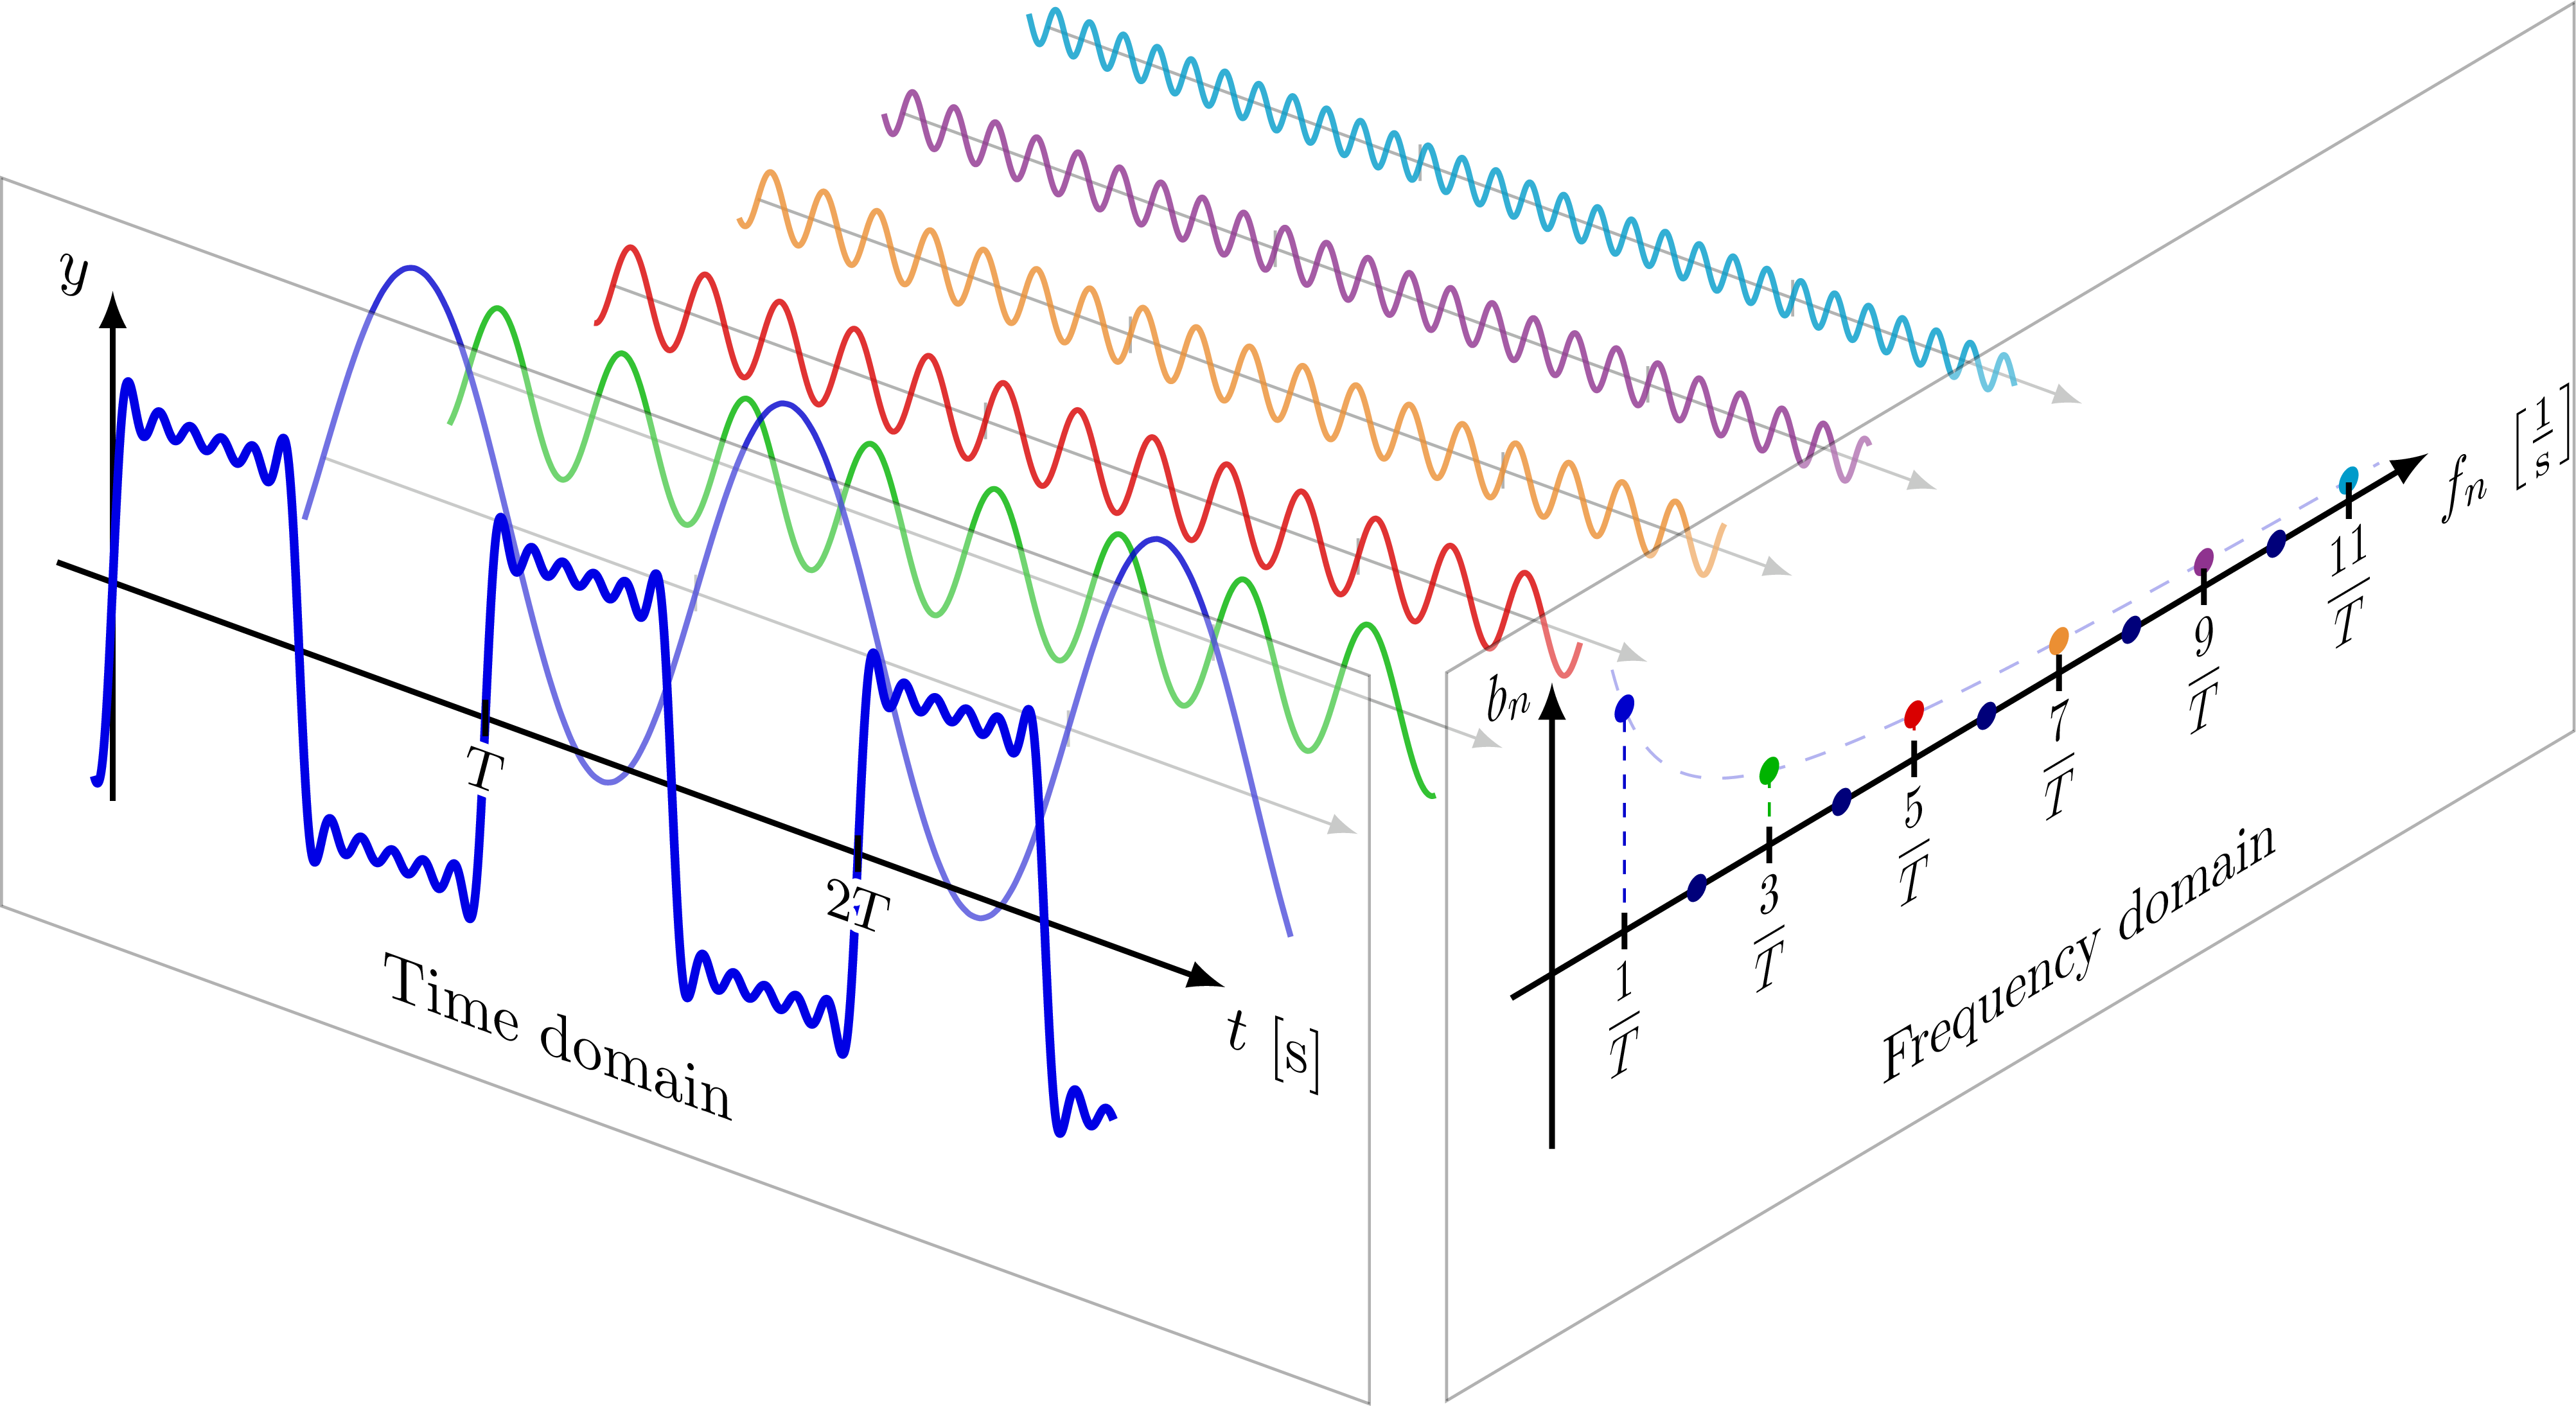
\includegraphics[width=0.9\textwidth]{imgs/investigacion/FourierSeries_Freq.png}
  \caption{Representación visual de la transformada de Fourier \cite{OGorman-2023}}
  \label{fig:fourier}
\end{figure}

\subsubsection{Espectrogramas}

La transformada de Fourier nos provee con las frecuencias de la canción,
pero la forma en la que estas pueden ser analizadas puede ser muy variada.
Una de las formas que existen para analizar estas frecuencias es a través de los
espectrogramas, los cuales son una representación visual de la cual se pueden
sacar distintas conclusiones del sonido que se tiene. Tratar la representación
visual de frecuencias como una imagen con textura permite reconocer la suavidad,
la regularidad, el contraste, entre otros \cite{Costa-2011}.

\begin{figure}[H]
  \centering
  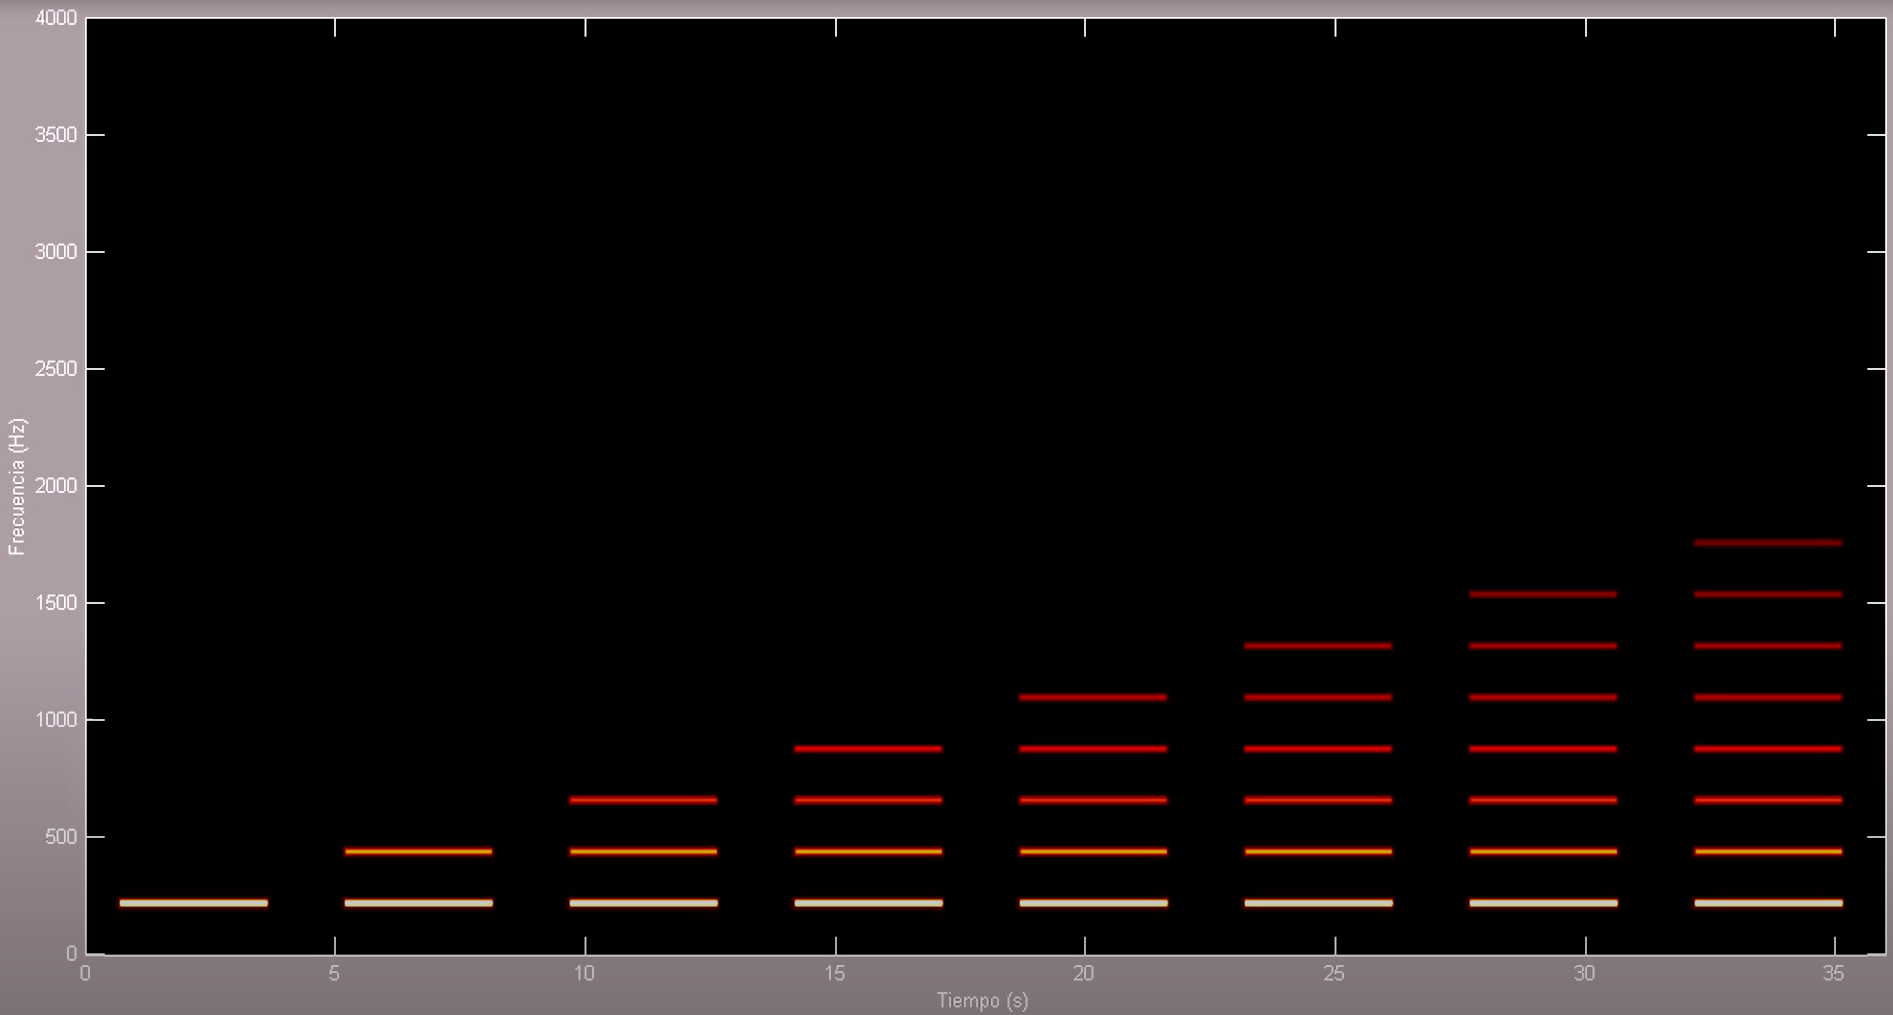
\includegraphics[width=0.8\textwidth]{imgs/investigacion/espectrogramas_01.png}
  \caption{Espectrograma de sonidos armónicos estables \cite{Colomer-01}}
  \label{fig:e1}
\end{figure}

\noindent La figura \ref{fig:e1} representa un espectrograma con
los componentes de la serie armónica. Se observan líneas bien definidas,
lo cual se asemejaría a lo que se busca en una canción instrumental.

\begin{figure}[H]
  \centering
  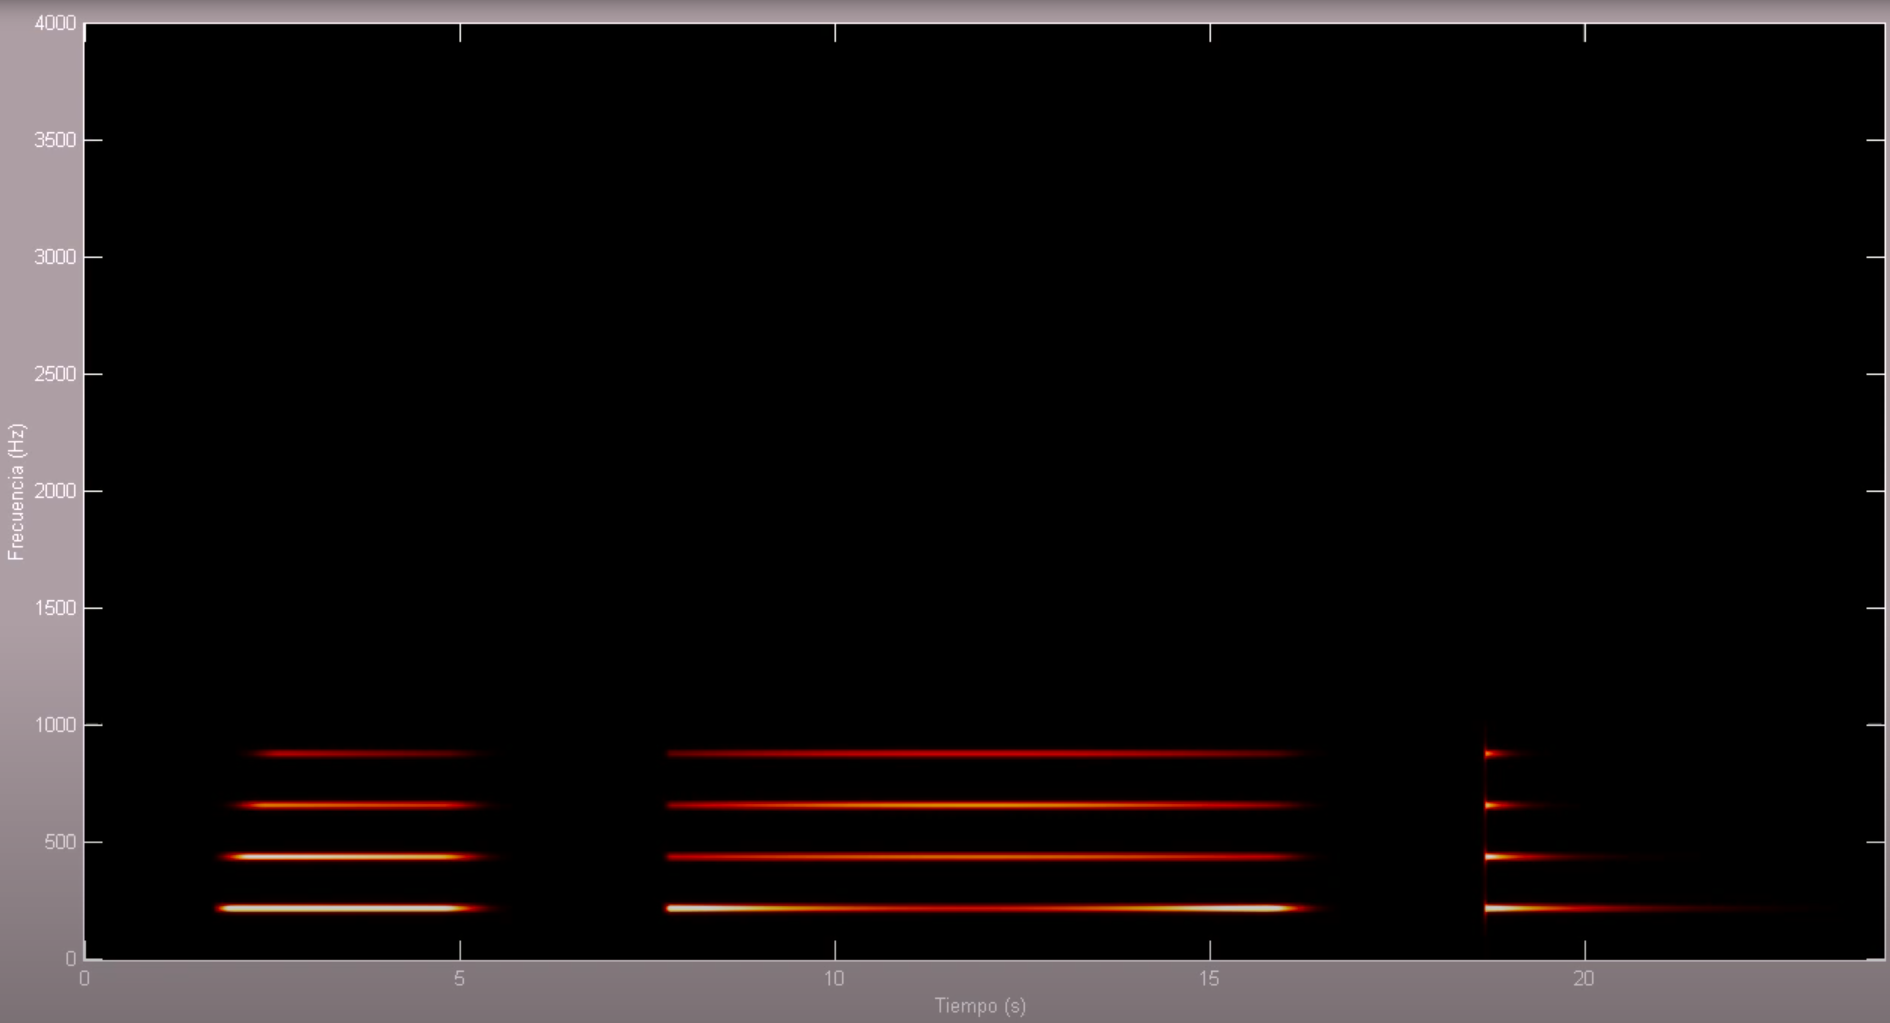
\includegraphics[width=0.8\textwidth]{imgs/investigacion/espectrogramas_02.png}
  \caption{Espectrograma de tres sonidos armónicos formados por
  componentes cuya amplitud evoluciona de diferentes formas \cite{Colomer-02}}
  \label{fig:e2}
\end{figure}

\noindent En la figura \ref{fig:e2} se tienen también sonidos armónicos,
solo que sus amplitudes cambian. A pesar de ello, se observan aún líneas
bien definidas, que también se podría esperar de las canciones instrumentales.

\begin{figure}[H]
  \centering
  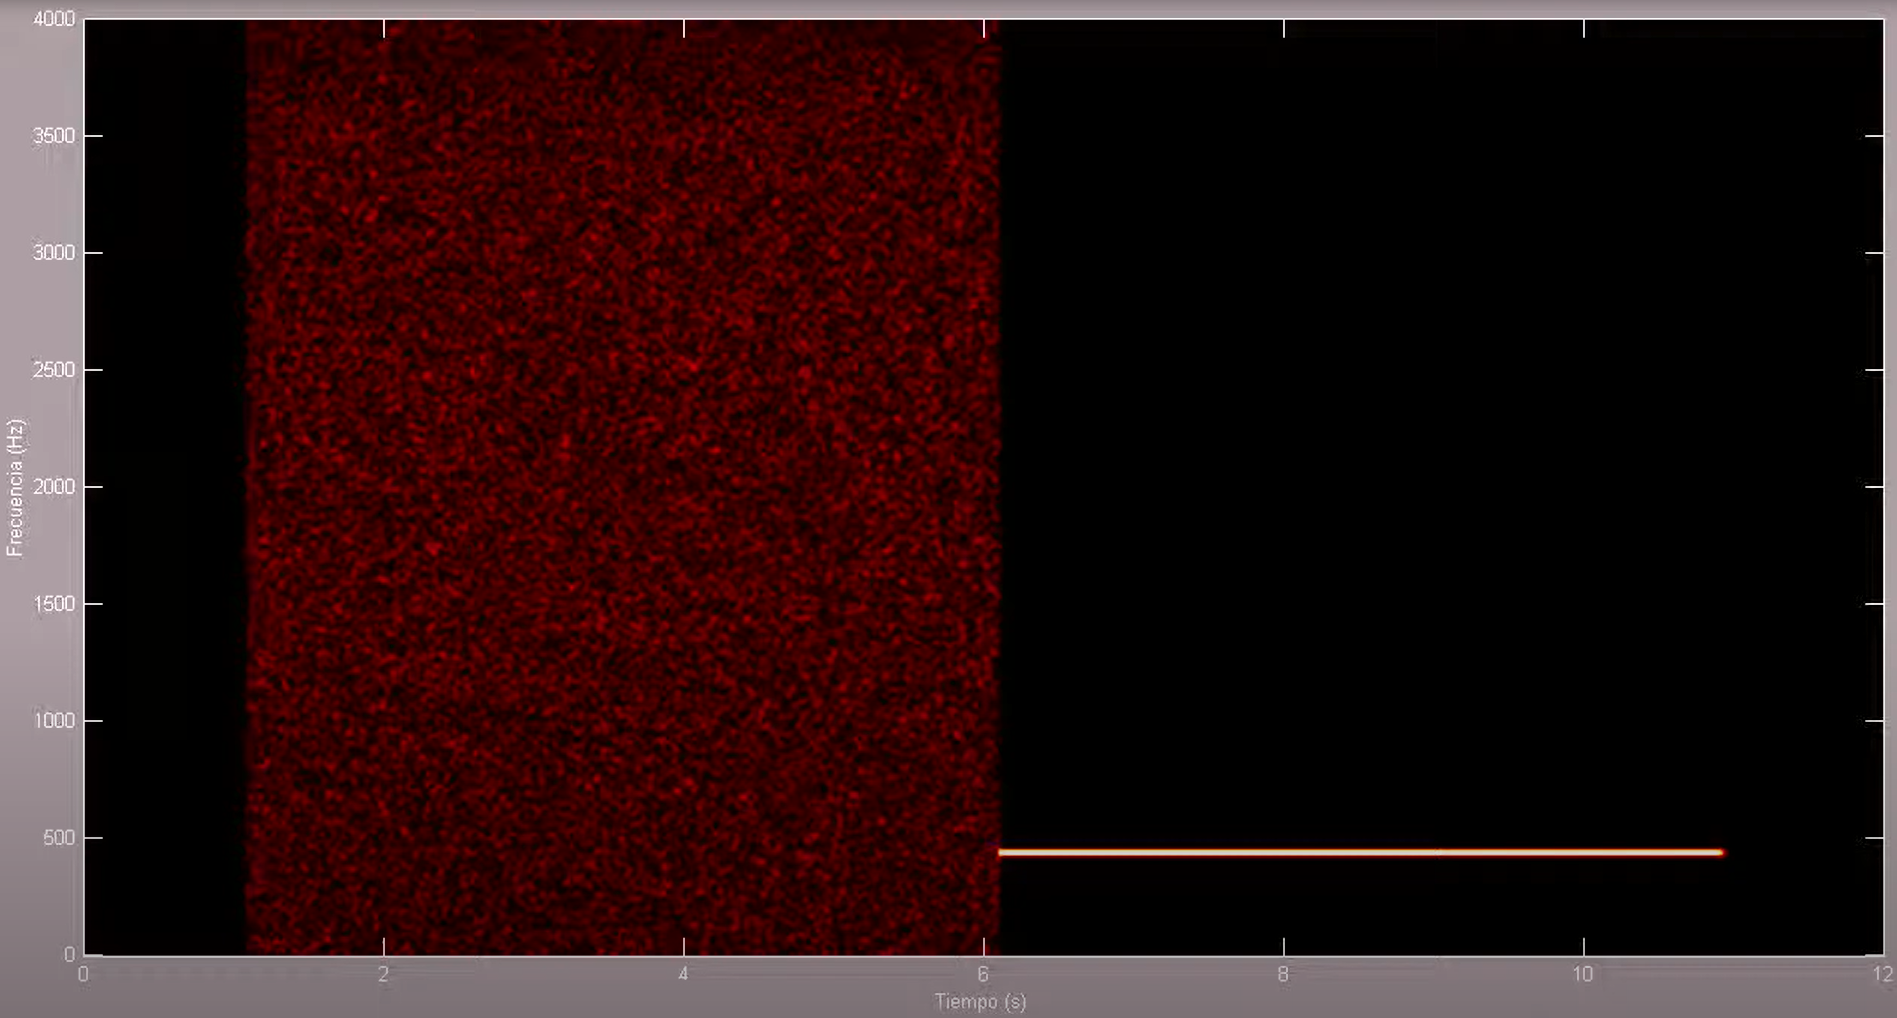
\includegraphics[width=0.8\textwidth]{imgs/investigacion/espectrogramas_04.png}
  \caption{Espectrograma de ruido blanco y sonido simple \cite{Colomer-04}}
  \label{fig:e4}
\end{figure}

\noindent En la figura \ref{fig:e4} se tiene ahora una comparación entre
el ruido blanco, el cual contiene a todas las frecuencias, y el sonido simple.
Se puede notar que cuando existe una gran combinación de frecuencias, el espectrograma
se encuentra muy saturado, mientras que cuando tenemos sonidos más puros, en el
espectrograma se tiene una línea definida.

\begin{figure}[H]
  \centering
  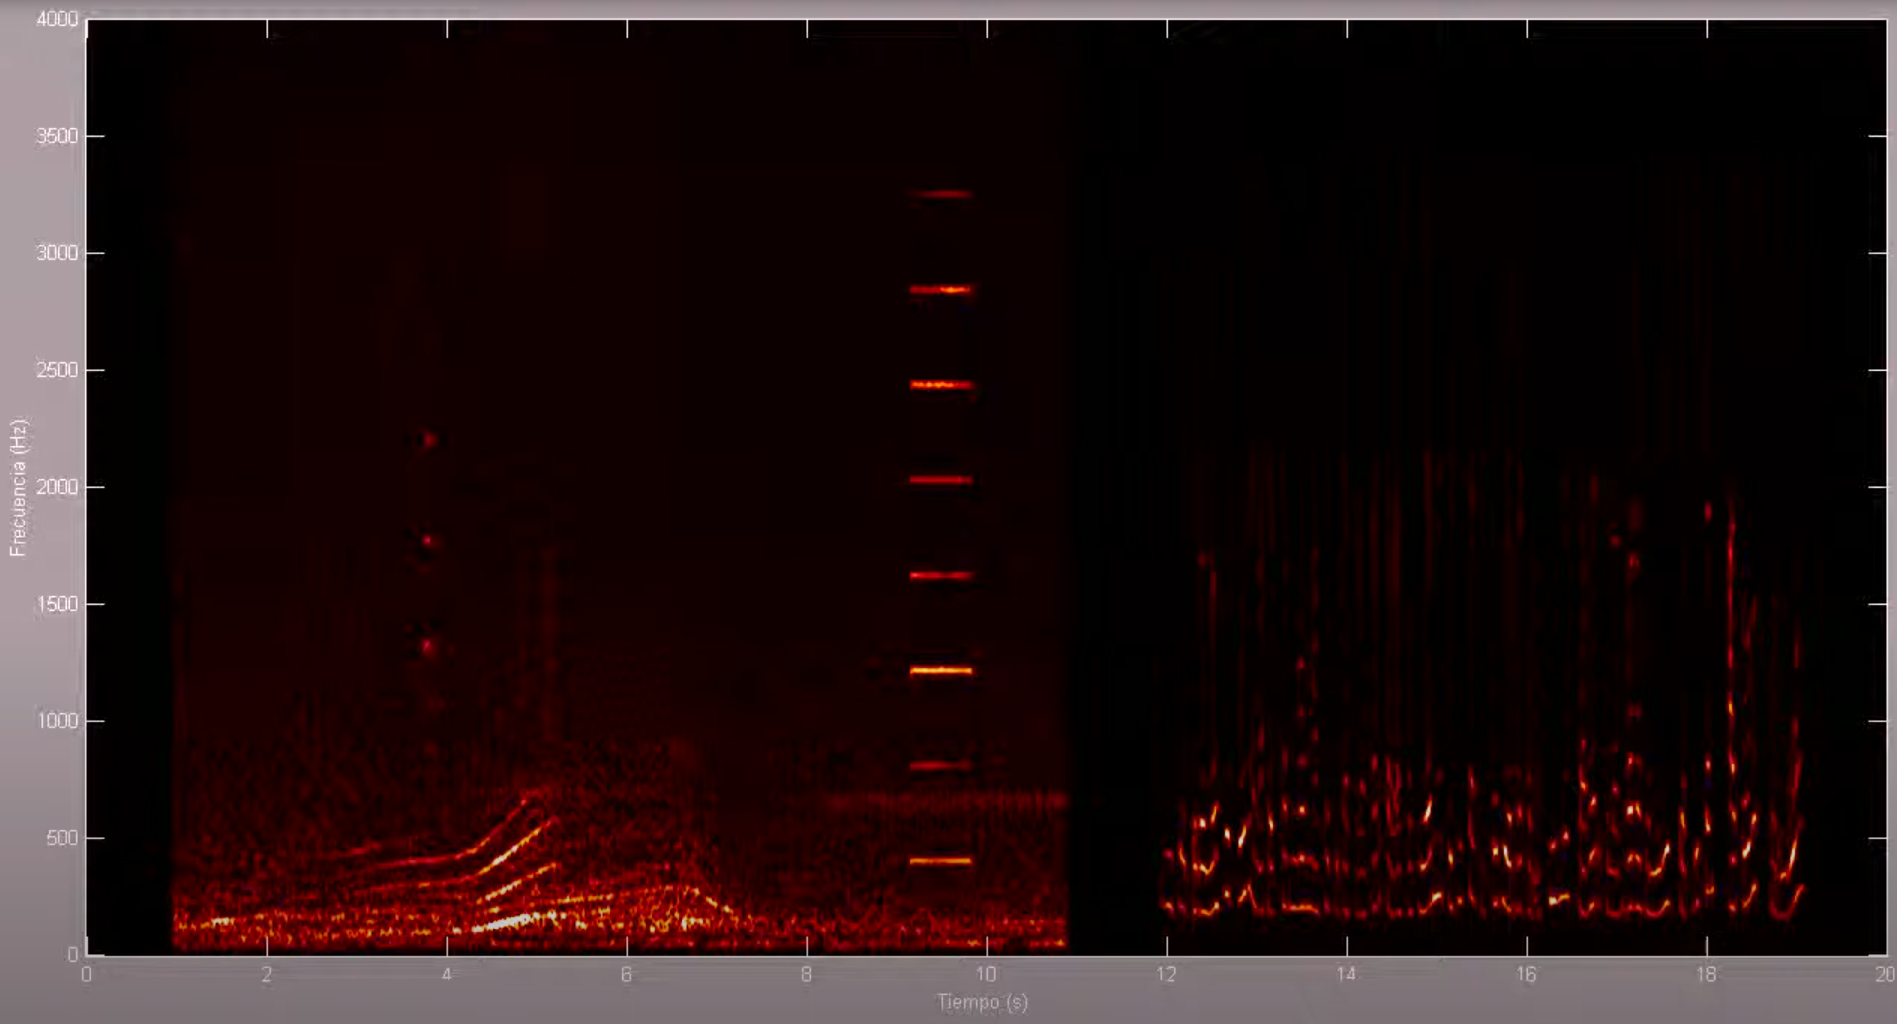
\includegraphics[width=0.8\textwidth]{imgs/investigacion/espectrogramas_05.png}
  \caption{Espectrograma de ruido de tráfico y de habla \cite{Colomer-05}}
  \label{fig:e5}
\end{figure}

\noindent En la figura \ref{fig:e5}, se tiene un espectograma que representa al
ruido del tráfico en la primera parte, y a una voz de un programa de radio en la segunda
mitad. Así como el ruido blanco, al tener una gran combinación de sonidos, la
parte del espectrograma con el ruido de tráfico está saturado en frecuencias bajas,
y en la parte derecha, hay varias líneas fragmentadas y que siguen distintas frecuencias.
Aquí ya no se llegan a ver líneas tan bien definidas como en las figuras
\ref{fig:e1} y \ref{fig:e2}, mas que a la mitad, con el
sonido de un claxon de auto, que se podría decir que es un sonido más definido
que el tráfico o la voz. \medskip

\noindent Utilizando estos ejemplos, se puede tener una intuición de qué esperar
en el espectrograma de cada género musical. Por un lado, con la música instrumental,
al no tener voces, y tener sonidos mezclados entre beats y los armónicos producidos
por los mismos instrumentos. Como no existe una gran mezcla de sonidos, el espectrograma
tendería a verse con líneas horizontales mejor definidas, como en las figuras
\ref{fig:e1} y \ref{fig:e2}. Por otro lado, en el género musical del reggaetón, se tiene
una gran combinación de sonidos, como el beat y los armónicos, además de tener una voz
que se podría asemejar a la segunda parte de la figura \ref{fig:e5}. Entonces el reggaetón
tendría una mayor combinación de ruidos, y su espectrograma tendría mucha textura.

\subsubsection{Espectro de frecuencias}

A pesar de que la voz sea una forma para identificar entre el reggaetón y la música
instrumental, no se tiene la seguridad de que esta sea inlcuida en los fragmentos
de canciones, y las formas de identificar la canción con el espectrograma sigue siendo
algo ambigua. Es por ello que, a la par, se pueden identificar ciertos rangos de frecuencias
que caracterizan a cada tipo de música.

El oído humano es capaz de escuchar frecuencias entre 20 y 20000 Hz, dentro de las
cuales se suelen hacer 3 categorías: bajos, medios y altos. A continuación se
presentan las subcategorías de estas, explicadas por Gleeson \cite{Gleeson-2024}:

\begin{itemize}
  \item Sub-bass (de los bajos): 20-60 Hz, es una frecuencia que suele sentirse más
  que escucharse.
  \item Mid-bass (o bass, de los bajos): 60-250 Hz, frecuencia baja que empieza a tener tonos más
  reconocibles.
  \item Low mids (de los medios): 250-500 Hz, suele representar una transición de las frecuencias
  bajas al rango medio.
  \item Center mids (o midrange, de los medios): 500-2000 Hz, en este rango de frecuencias
  se suelen encontrar los armónicos y fundamentales de las partes más importantes de las
  canciones.
  \item Upper mids (de los medios): 2000-4000 Hz, un rango de frecuencia que suele consistir en
  armónicos, detalles del timbre y sonidos transitorios.
  \item Presence (de los altos): 4000-6000 Hz, que consiste principalmente por frecuencias
  armónicas.
  \item Brilliance (de los altos): 6000-20000 Hz, que suele indicar el timbre general del sonido,
  mas no su tonalidad.
\end{itemize}

Estilos de música como el reggae, dub y dancehall Jamaiquinos, el hip-hop, la cumbia,
el reggaetón, el Miami bass, entre otros, utilizan una gran cantidad de sonidos de baja
frecuencia. Las bandas de frecuencias por debajo de los 100 Hz, en los límites
de lo audible, alteran la realidad física al vibrar \cite{fink-2018}.

De acuerdo con García\cite{Garcia-2016}, el reggaetón es uno de los géneros orientados al
bass, cuyos beats utilizan frecuencias alrededor de los 20 Hz y producen una experiencia
energizante, opresiva, impulsiva, desorientadora, entre otros. Es a través de estas
frecuencias se involucran los sentidos hápticos al escuchar y bailar este tipo de música.

Tanto García\cite{Garcia-2016} como Fink\cite{fink-2018} coinciden en que el reggaetón
utiliza muchas frecuencias bajas para generar el efecto querido en el oyente. La música
de reggaetón se presta mucho para bailar, mientras que la música instrumental no presenta
este tipo de beats que hacen vibrar al cuerpo, no generando así el mismo efecto
que el reggaetón en el oyente.

\newpage
\section{Resultados}

\textbf{\large{Canción 1}}

\begin{figure}[H]
  \centering
  \begin{minipage}{.4\linewidth}
    \centering
    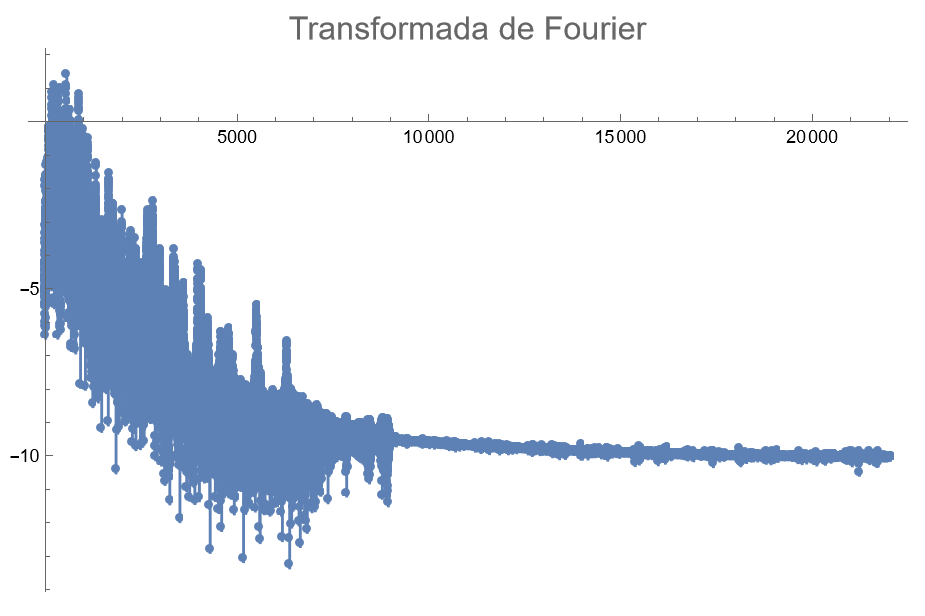
\includegraphics[width=\linewidth]{imgs/Cancion1/transformada.png}
    \captionof{figure}{Logaritmo de la transformada de Fourier de la canción 1}
    \label{fig:01a}
  \end{minipage}
  \begin{minipage}{0.07\textwidth}\end{minipage}
  \begin{minipage}{.47\linewidth}
    \centering
    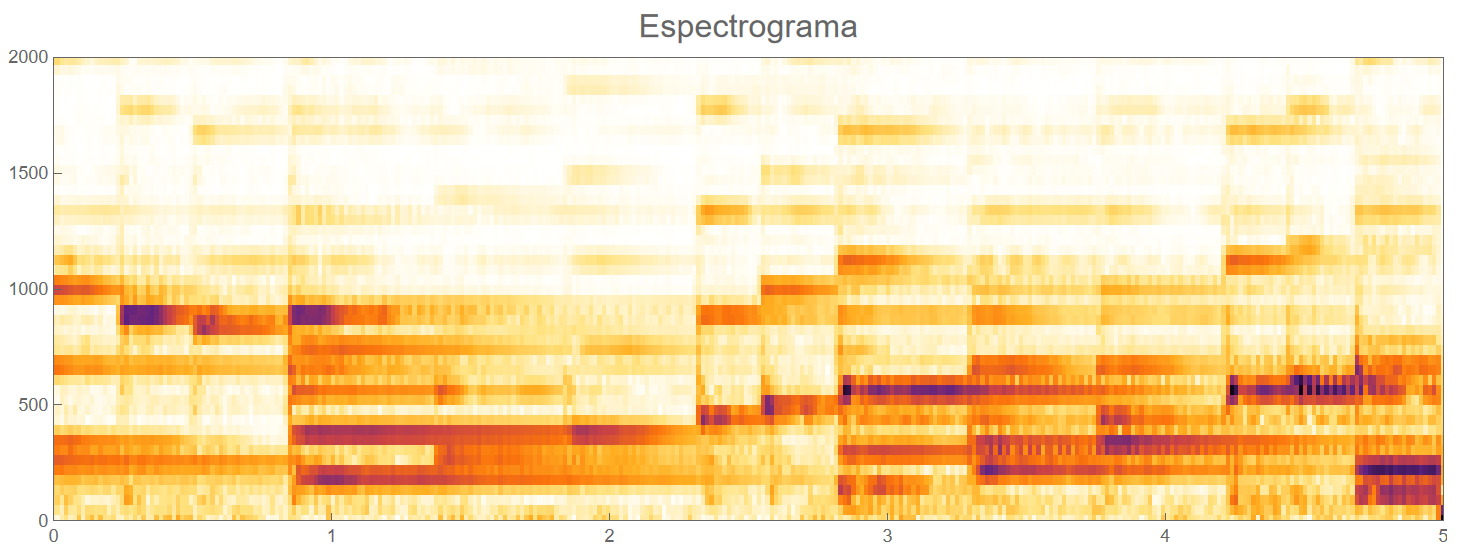
\includegraphics[width=\linewidth]{imgs/Cancion1/espectrograma.png}
    \caption{Espectrograma de la canción 1}
    \label{fig:01i}
  \end{minipage}
\end{figure}
\begin{figure}[H]
  \centering
  \begin{minipage}{.3\textwidth}
    \centering
    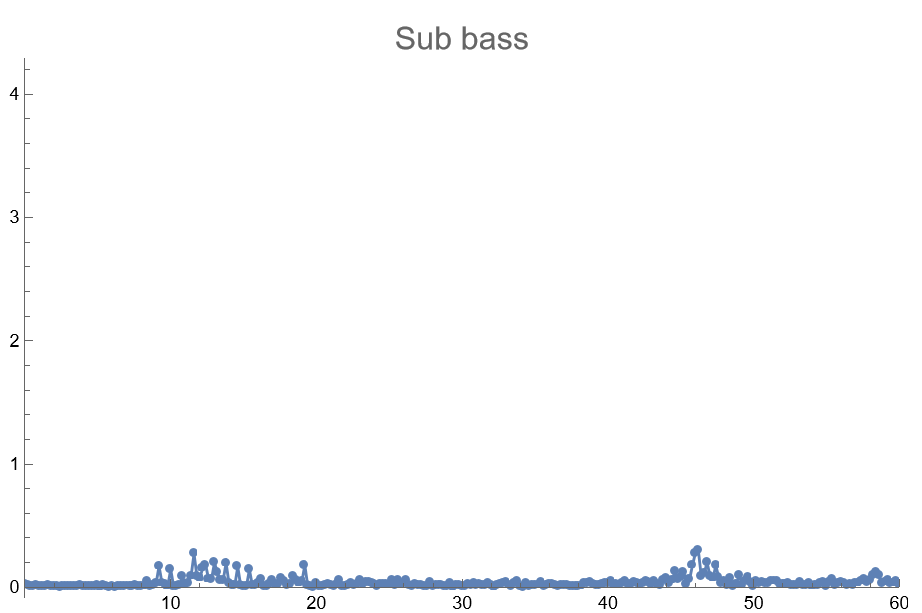
\includegraphics[width=.9\linewidth]{imgs/Cancion1/subbass.png}
  \end{minipage}
  \begin{minipage}{0.03\textwidth}\end{minipage}
  \begin{minipage}{.3\textwidth}
    \centering
    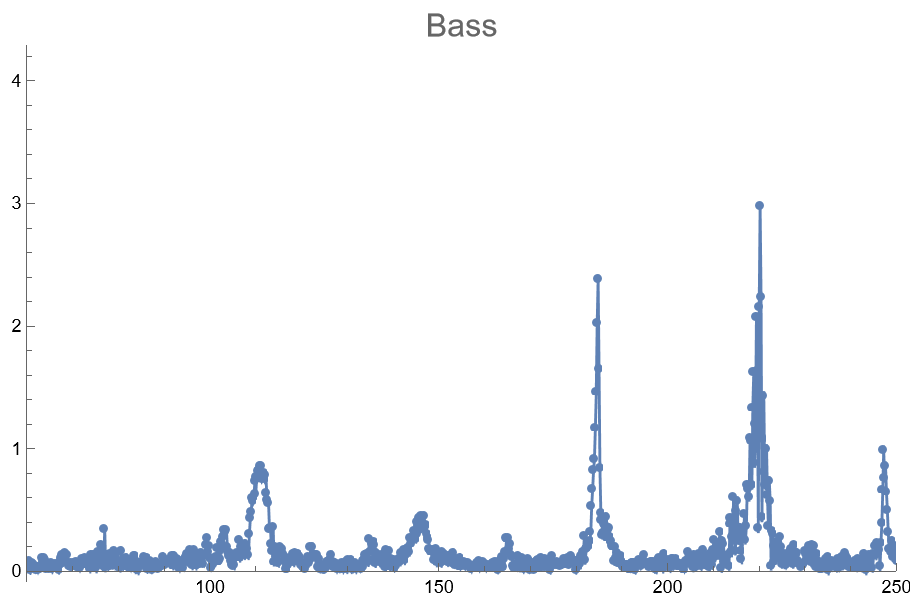
\includegraphics[width=.9\linewidth]{imgs/Cancion1/bass.png}
  \end{minipage} \medskip \\
  \begin{minipage}{.3\textwidth}
    \centering
    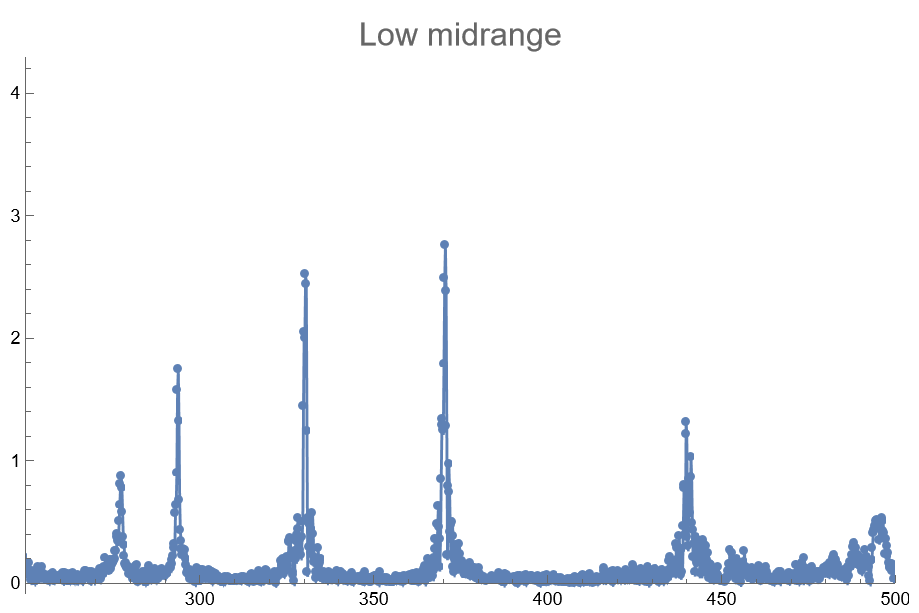
\includegraphics[width=.9\linewidth]{imgs/Cancion1/lowmid.png}
  \end{minipage}
  \begin{minipage}{0.03\textwidth}\end{minipage}
  \begin{minipage}{.3\textwidth}
    \centering
    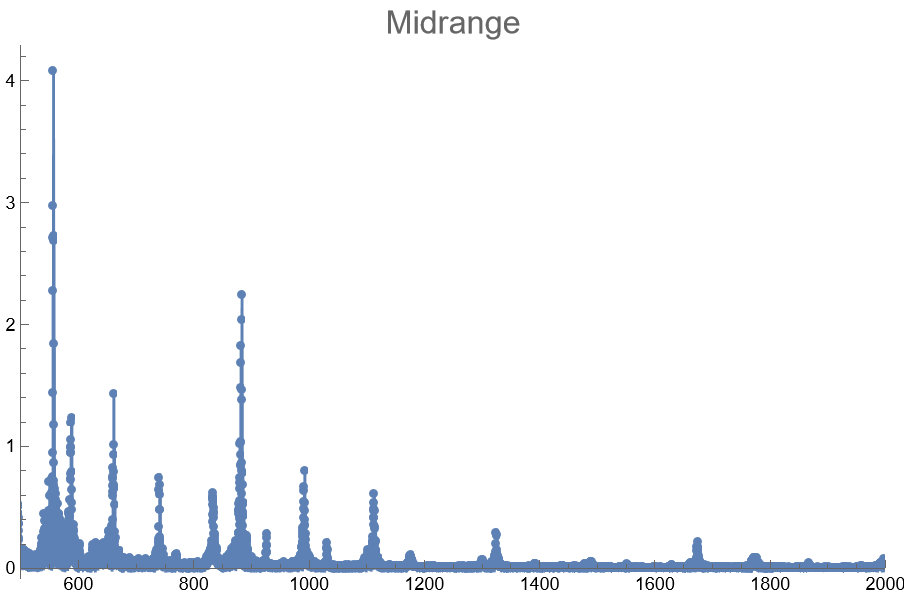
\includegraphics[width=.9\linewidth]{imgs/Cancion1/mid.png}
  \end{minipage}
  \begin{minipage}{0.03\textwidth}\end{minipage}
  \begin{minipage}{.3\textwidth}
    \centering
    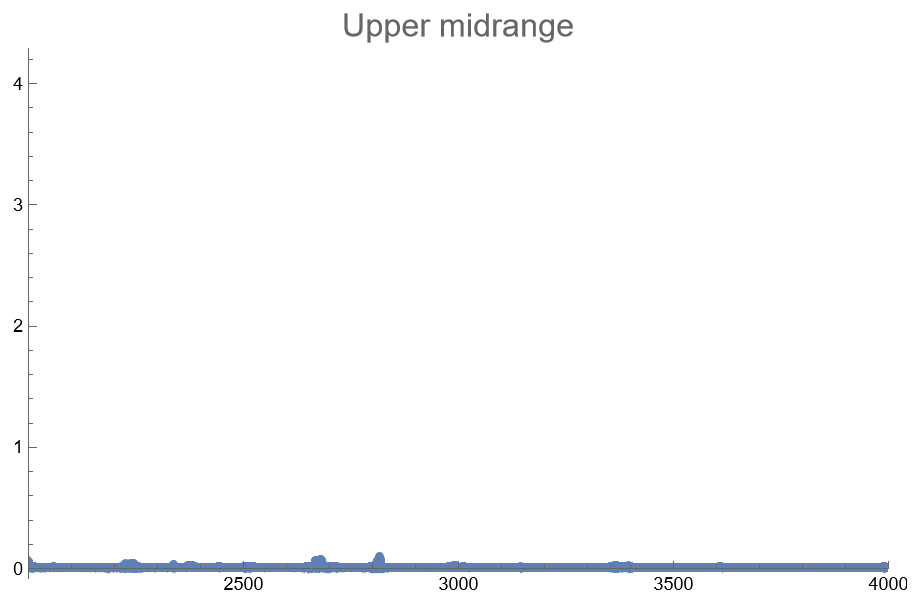
\includegraphics[width=.9\linewidth]{imgs/Cancion1/upmid.png}
  \end{minipage} \medskip \\
  \begin{minipage}{.3\textwidth}
    \centering
    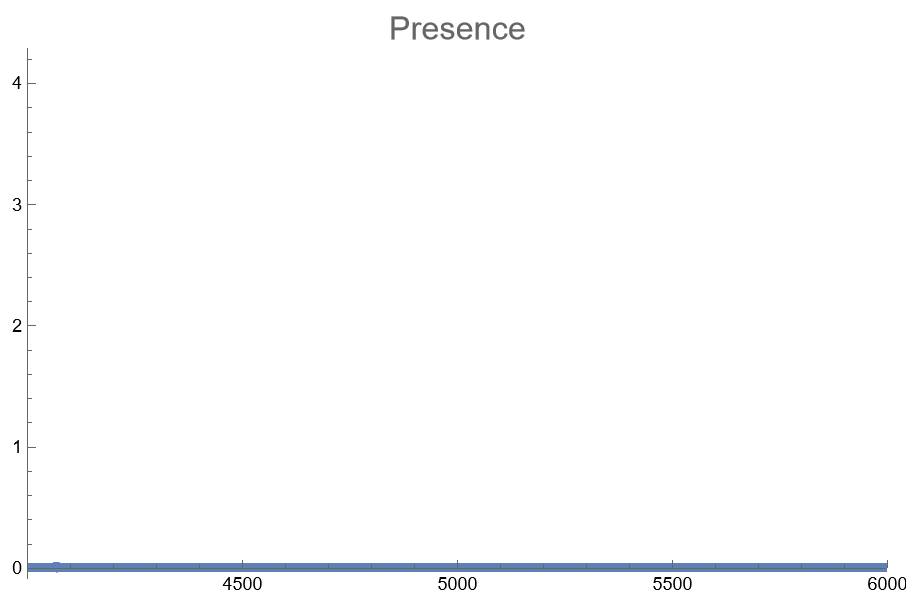
\includegraphics[width=.9\linewidth]{imgs/Cancion1/presence.png}
  \end{minipage}
  \begin{minipage}{0.03\textwidth}\end{minipage}
  \begin{minipage}{.3\textwidth}
    \centering
    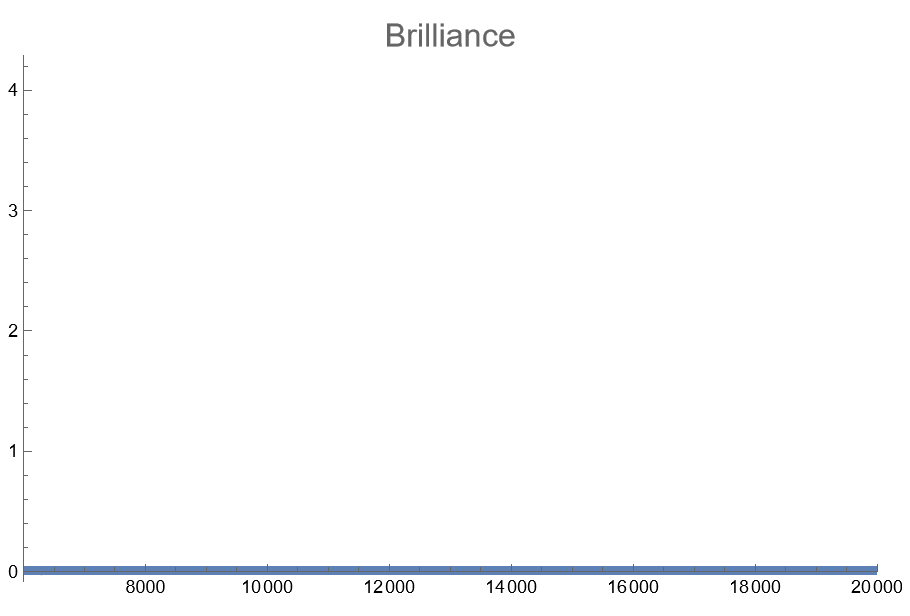
\includegraphics[width=.9\linewidth]{imgs/Cancion1/brilliance.png}
  \end{minipage}
  \caption{Espectro de frecuencias de la canción 1}
  \label{fig:esp01}
\end{figure}

\textbf{Clasificación}: Instrumental

\textbf{Justificación}: Observando el espectro de frecuencias de la canción,
se ve una mayor predominancia en frecuencias que se encuentran en bass, low
midrange y en midrange. Al no incluir un subbass tan marcado, clasificamos
a esta canción como instrumental. Asimismo, observamos que el espectrograma no
parece presentar mucho ruido, y se parece más a los espectrogramas de ejemplo
de sonidos armónicos (como en la Figura \ref{fig:e2}), confirmando nuestra
clasificación.

\newpage

\textbf{\large{Canción 2}}

\begin{figure}[H]
  \centering
  \begin{minipage}{.4\linewidth}
    \centering
    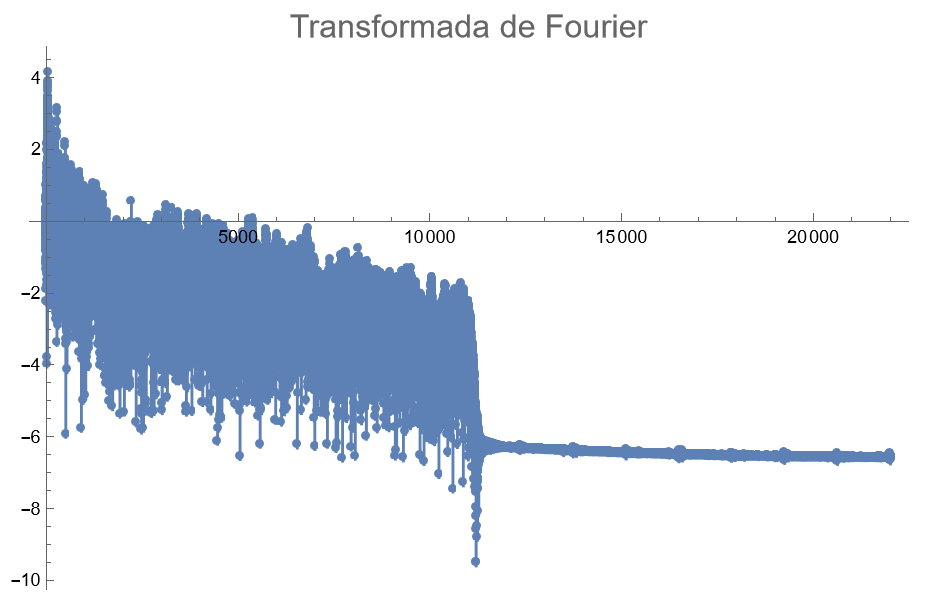
\includegraphics[width=\linewidth]{imgs/Cancion2/transformada.png}
    \captionof{figure}{Logaritmo de la transformada de Fourier de la canción 2}
    \label{fig:02a}
  \end{minipage}
  \begin{minipage}{0.07\textwidth}\end{minipage}
  \begin{minipage}{.47\linewidth}
    \centering
    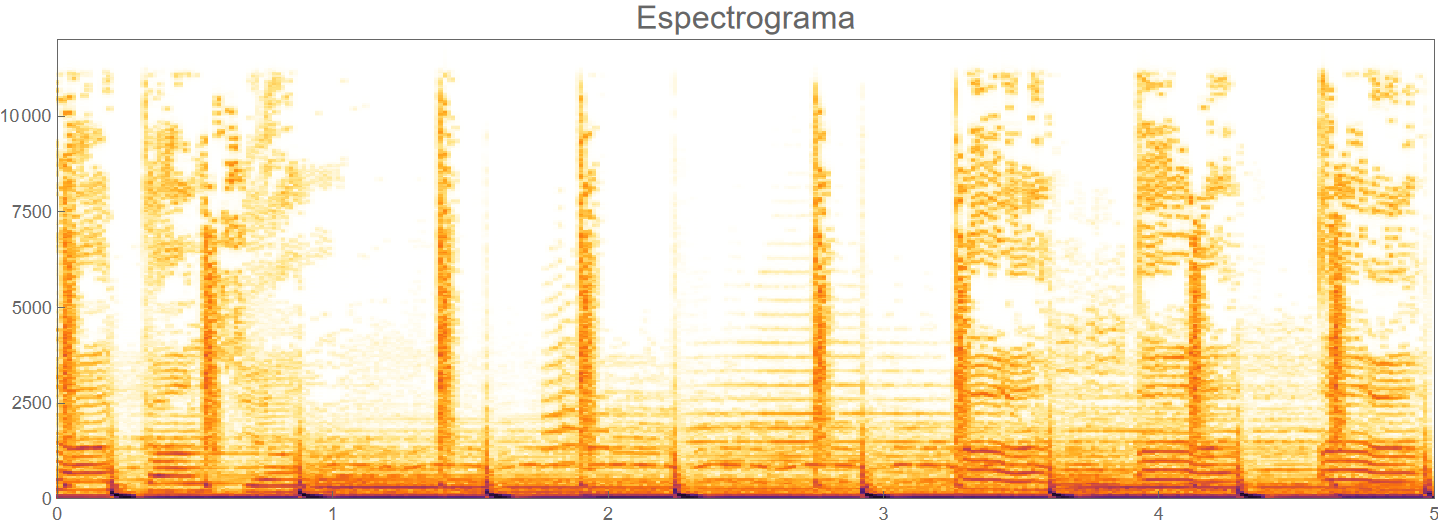
\includegraphics[width=\linewidth]{imgs/Cancion2/espectrograma.png}
    \caption{Espectrograma de la canción 2}
    \label{fig:02i}
  \end{minipage}
\end{figure}
\begin{figure}[H]
  \centering
  \begin{minipage}{.3\textwidth}
    \centering
    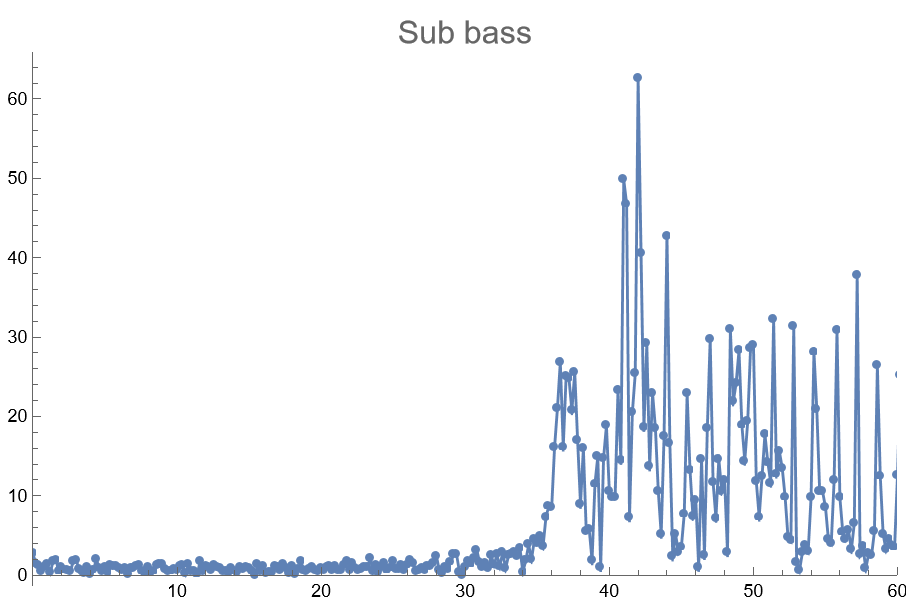
\includegraphics[width=.9\linewidth]{imgs/Cancion2/subbass.png}
  \end{minipage}
  \begin{minipage}{0.03\textwidth}\end{minipage}
  \begin{minipage}{.3\textwidth}
    \centering
    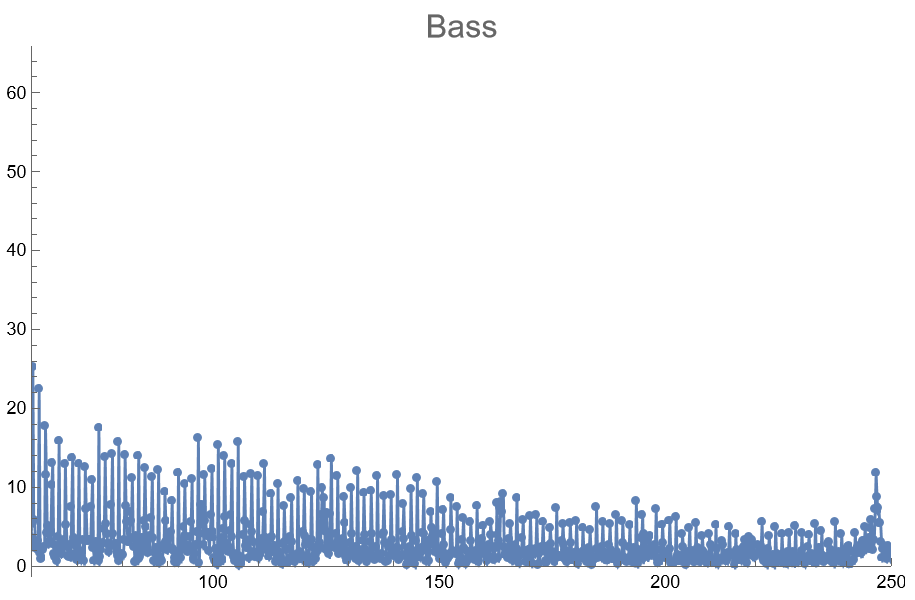
\includegraphics[width=.9\linewidth]{imgs/Cancion2/bass.png}
  \end{minipage} \medskip \\
  \begin{minipage}{.3\textwidth}
    \centering
    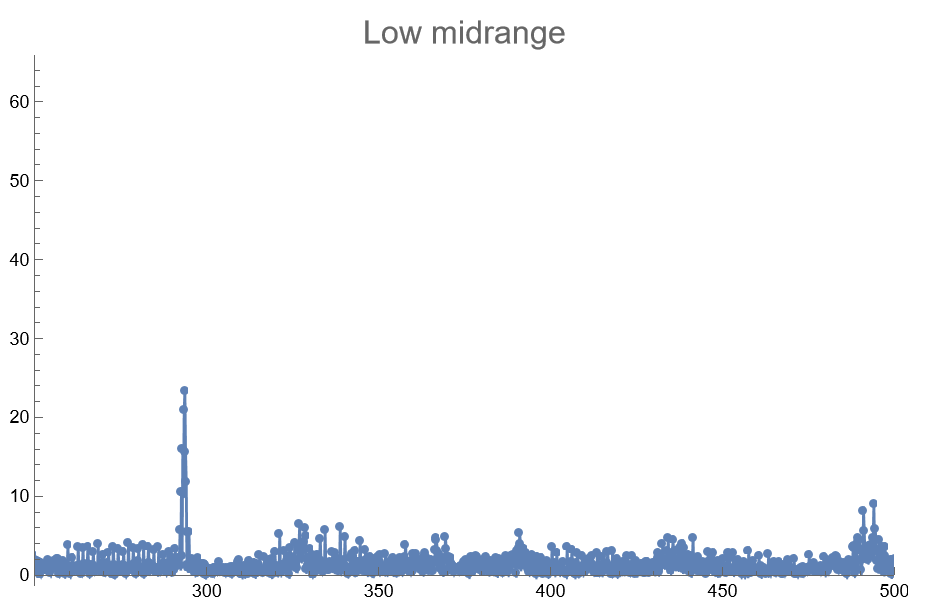
\includegraphics[width=.9\linewidth]{imgs/Cancion2/lowmid.png}
  \end{minipage}
  \begin{minipage}{0.03\textwidth}\end{minipage}
  \begin{minipage}{.3\textwidth}
    \centering
    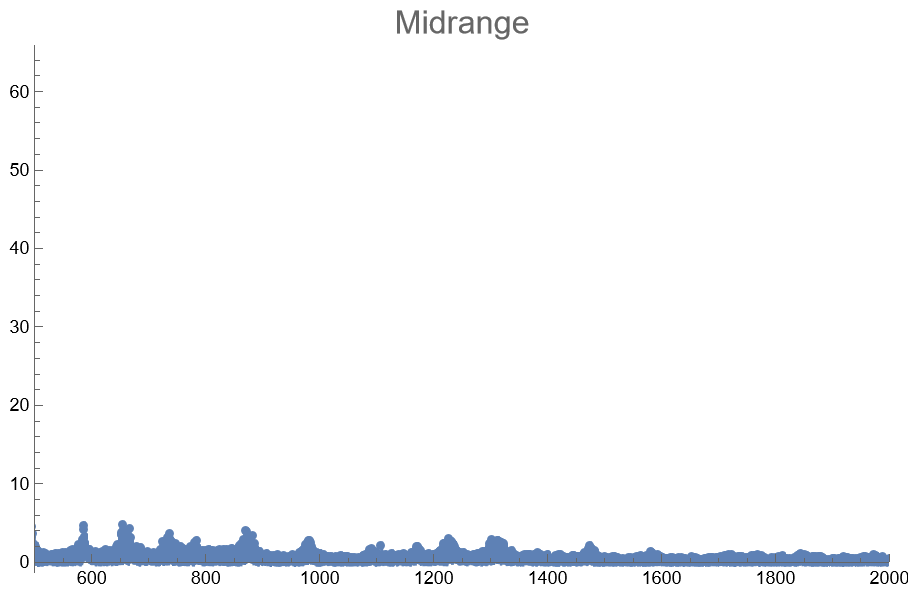
\includegraphics[width=.9\linewidth]{imgs/Cancion2/mid.png}
  \end{minipage}
  \begin{minipage}{0.03\textwidth}\end{minipage}
  \begin{minipage}{.3\textwidth}
    \centering
    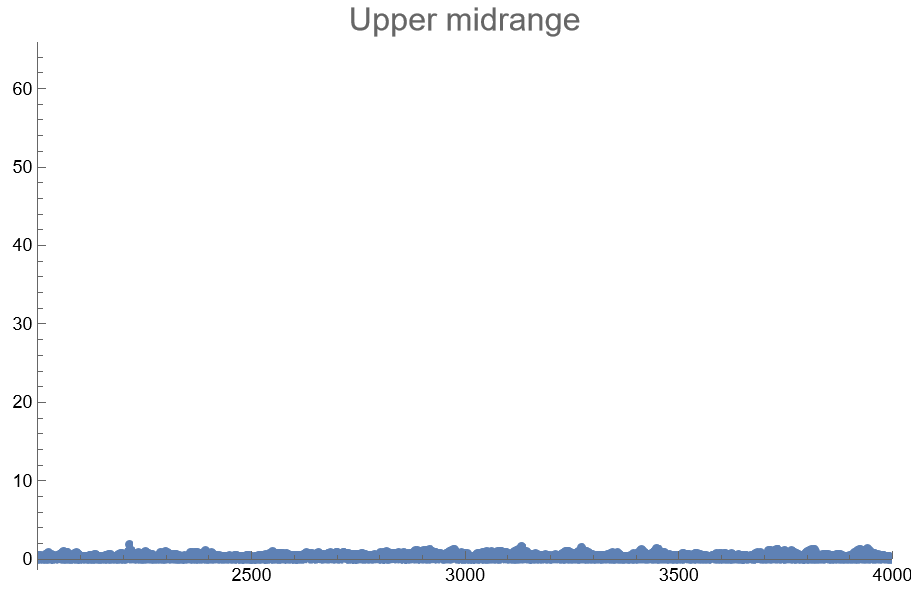
\includegraphics[width=.9\linewidth]{imgs/Cancion2/upmid.png}
  \end{minipage} \medskip \\
  \begin{minipage}{.3\textwidth}
    \centering
    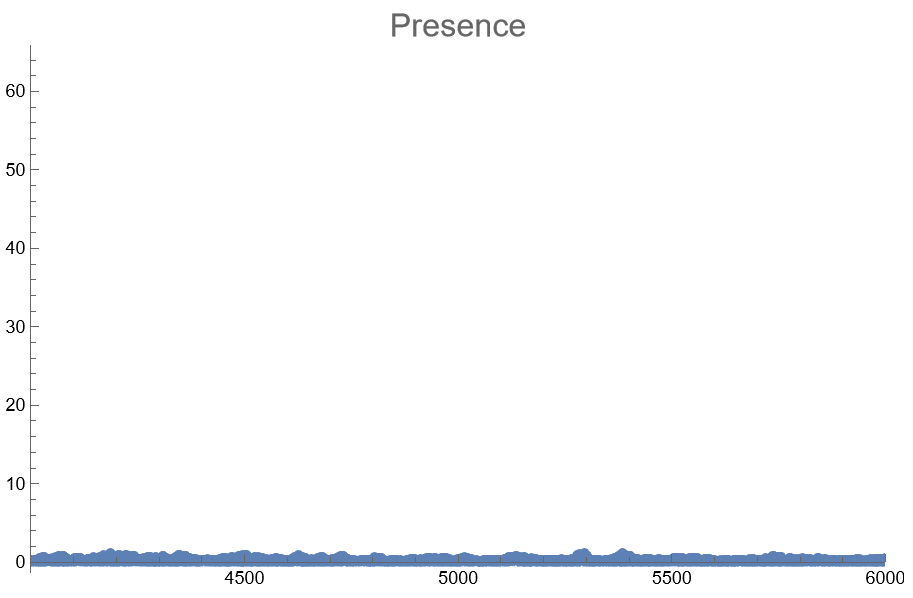
\includegraphics[width=.9\linewidth]{imgs/Cancion2/presence.png}
  \end{minipage}
  \begin{minipage}{0.03\textwidth}\end{minipage}
  \begin{minipage}{.3\textwidth}
    \centering
    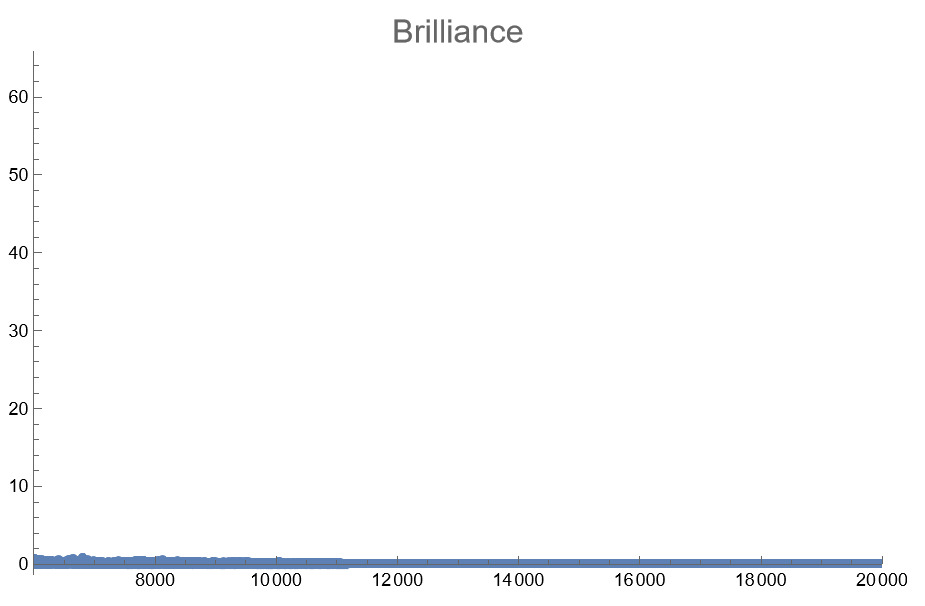
\includegraphics[width=.9\linewidth]{imgs/Cancion2/brilliance.png}
  \end{minipage}
  \caption{Espectro de frecuencias de la canción 2}
  \label{fig:esp02}
\end{figure}

\textbf{Clasificación}: Reggaetón

\textbf{Justificación}: A diferencia de la canción anterior, en esta
observamos que las frecuencias que dominan en esta canción son subbass y 
bass. Es por ello que clasificamos a esta canción como reggaetón, por su
baja frecuencia. Asimismo, observando el espectrograma, existe mucho ruido
que no parece ser tan armónico, que sería más probable a ser reggaetón que
música instrumental.

\newpage

\textbf{\large{Canción 3}}

\begin{figure}[H]
  \centering
  \begin{minipage}{.4\linewidth}
    \centering
    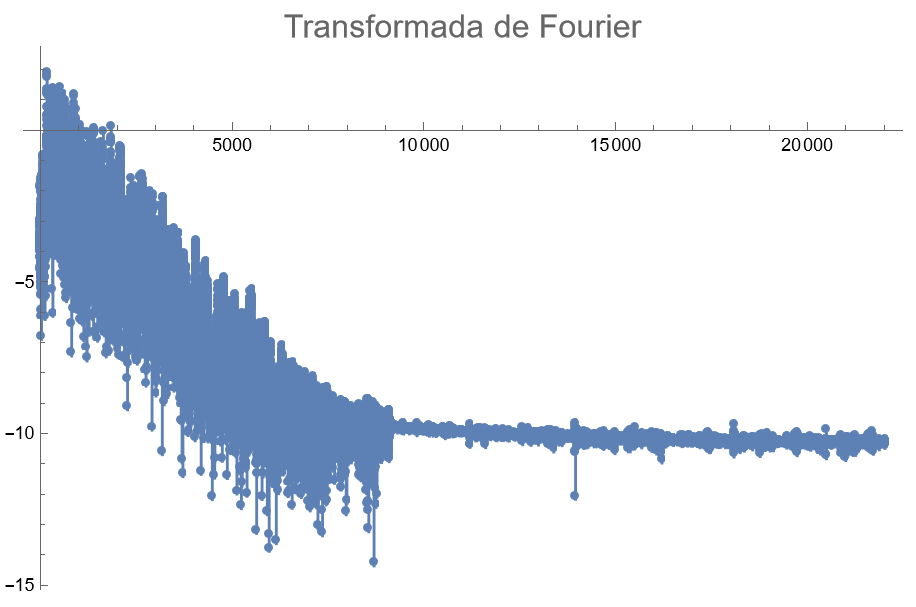
\includegraphics[width=\linewidth]{imgs/Cancion3/transformada.png}
    \captionof{figure}{Logaritmo de la transformada de Fourier de la canción 3}
    \label{fig:03a}
  \end{minipage}
  \begin{minipage}{0.07\textwidth}\end{minipage}
  \begin{minipage}{.47\linewidth}
    \centering
    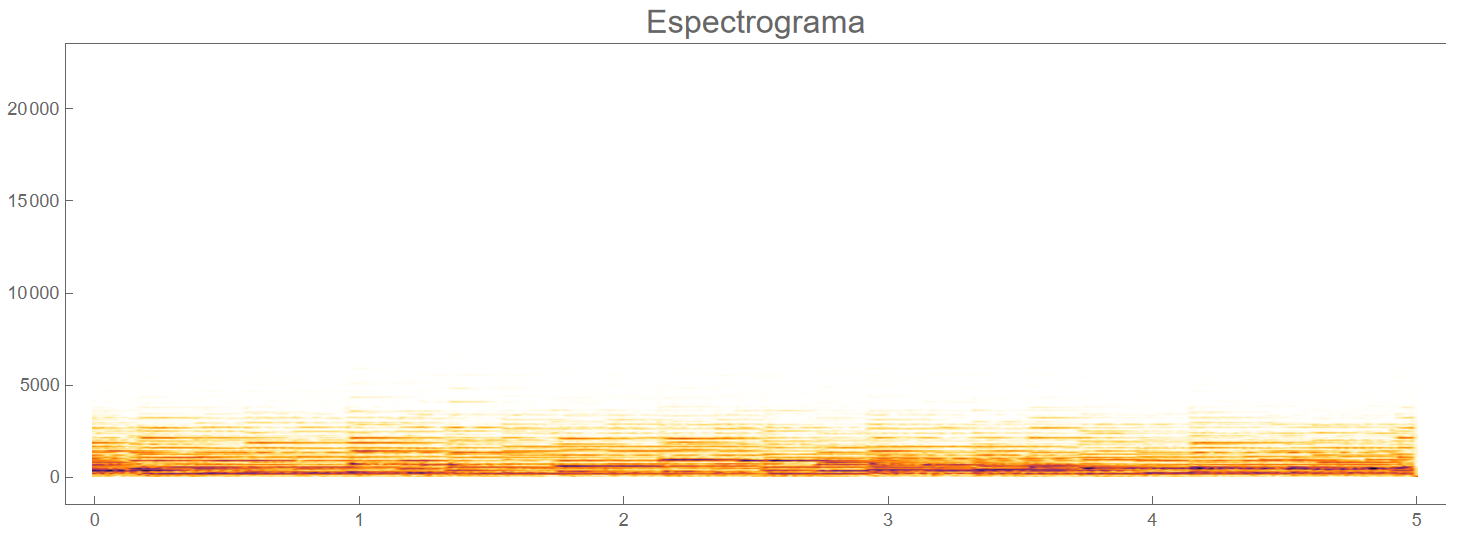
\includegraphics[width=\linewidth]{imgs/Cancion3/espectrograma.png}
    \caption{Espectrograma de la canción 3}
    \label{fig:03i}
  \end{minipage}
\end{figure}
\begin{figure}[H]
  \centering
  \begin{minipage}{.3\textwidth}
    \centering
    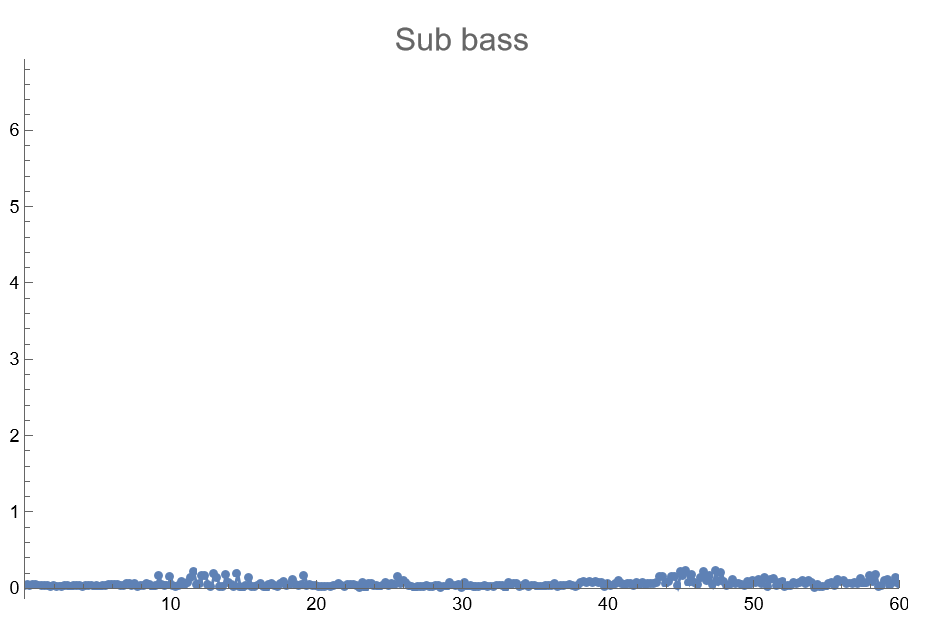
\includegraphics[width=.9\linewidth]{imgs/Cancion3/subbass.png}
  \end{minipage}
  \begin{minipage}{0.03\textwidth}\end{minipage}
  \begin{minipage}{.3\textwidth}
    \centering
    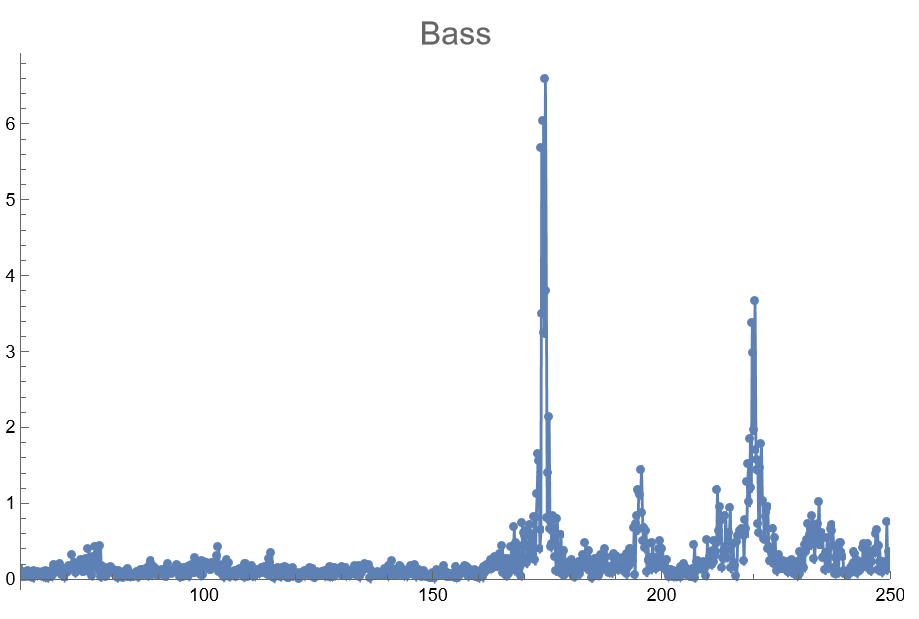
\includegraphics[width=.9\linewidth]{imgs/Cancion3/bass.png}
  \end{minipage} \medskip \\
  \begin{minipage}{.3\textwidth}
    \centering
    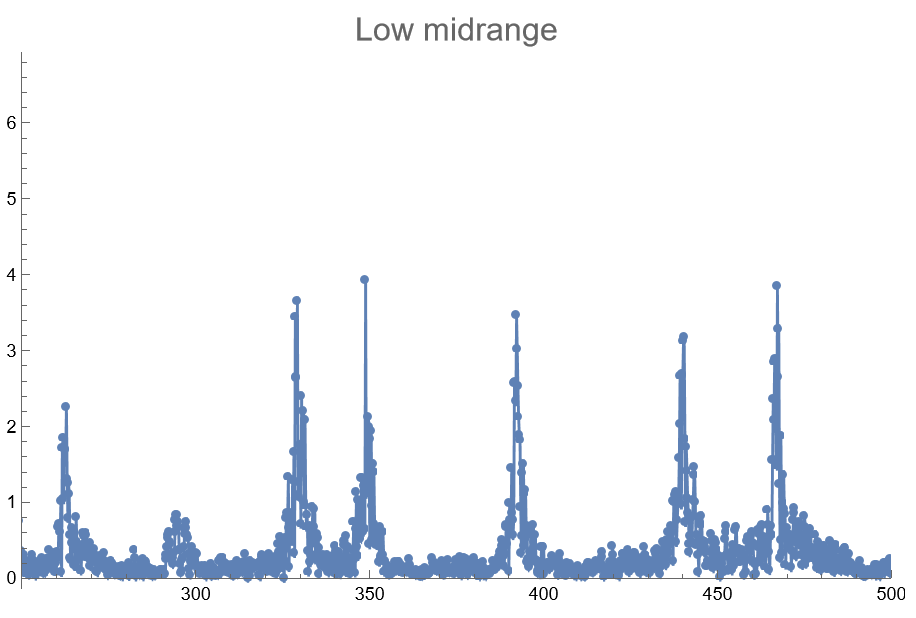
\includegraphics[width=.9\linewidth]{imgs/Cancion3/lowmid.png}
  \end{minipage}
  \begin{minipage}{0.03\textwidth}\end{minipage}
  \begin{minipage}{.3\textwidth}
    \centering
    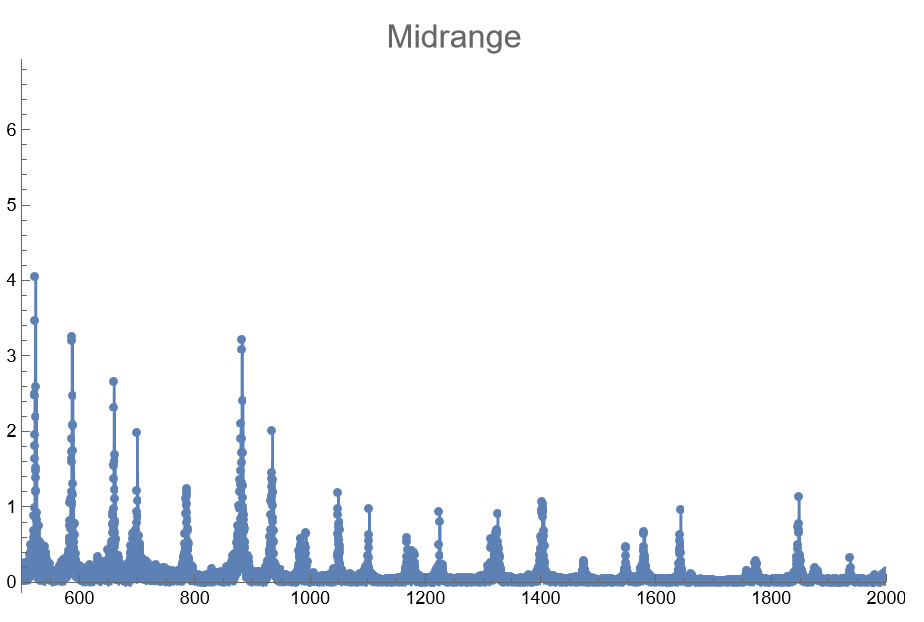
\includegraphics[width=.9\linewidth]{imgs/Cancion3/mid.png}
  \end{minipage}
  \begin{minipage}{0.03\textwidth}\end{minipage}
  \begin{minipage}{.3\textwidth}
    \centering
    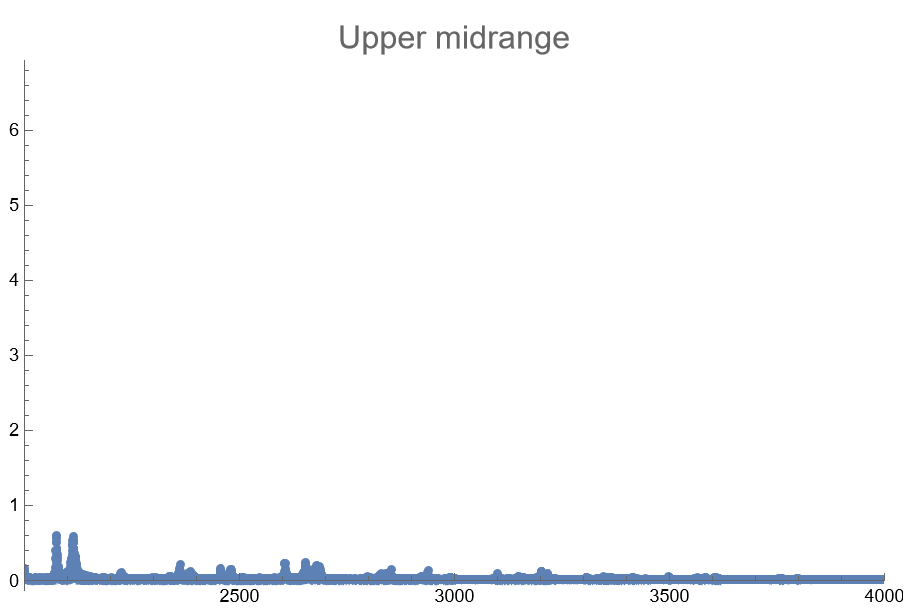
\includegraphics[width=.9\linewidth]{imgs/Cancion3/upmid.png}
  \end{minipage} \medskip \\
  \begin{minipage}{.3\textwidth}
    \centering
    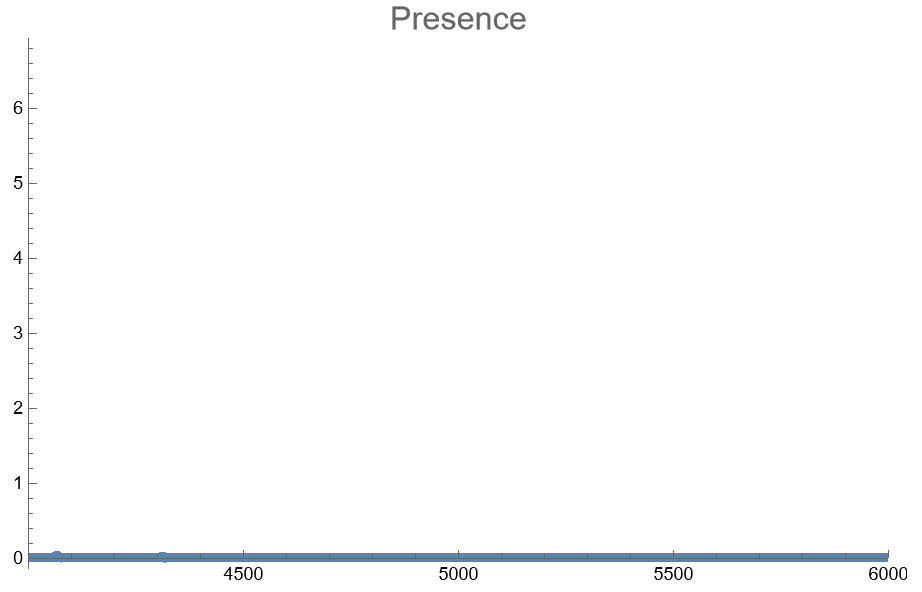
\includegraphics[width=.9\linewidth]{imgs/Cancion3/presence.png}
  \end{minipage}
  \begin{minipage}{0.03\textwidth}\end{minipage}
  \begin{minipage}{.3\textwidth}
    \centering
    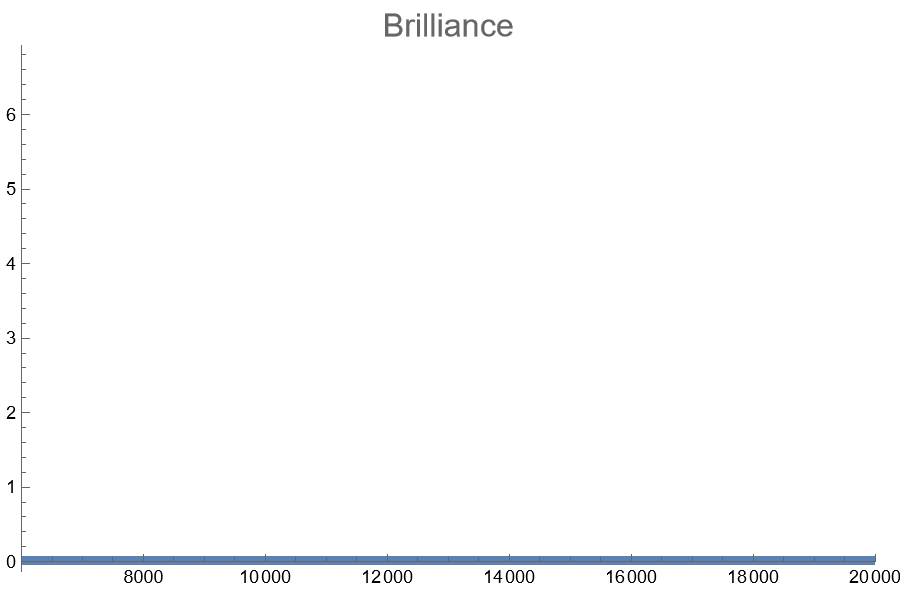
\includegraphics[width=.9\linewidth]{imgs/Cancion3/brilliance.png}
  \end{minipage}
  \caption{Espectro de frecuencias de la canción 3}
  \label{fig:esp03}
\end{figure}

\textbf{Clasificación}: Instrumental

\textbf{Justificación}: Esta canción presenta más frecuencias entre bass
y midrange dentro de su espectro de frecuencias. Al no presentar tanto subbass,
la clasificamos como instrumental. Observando el espectrograma, también observamos
que las frecuencias se ven más armónicas.

\newpage

\textbf{\large{Canción 4}}

\begin{figure}[H]
  \centering
  \begin{minipage}{.4\linewidth}
    \centering
    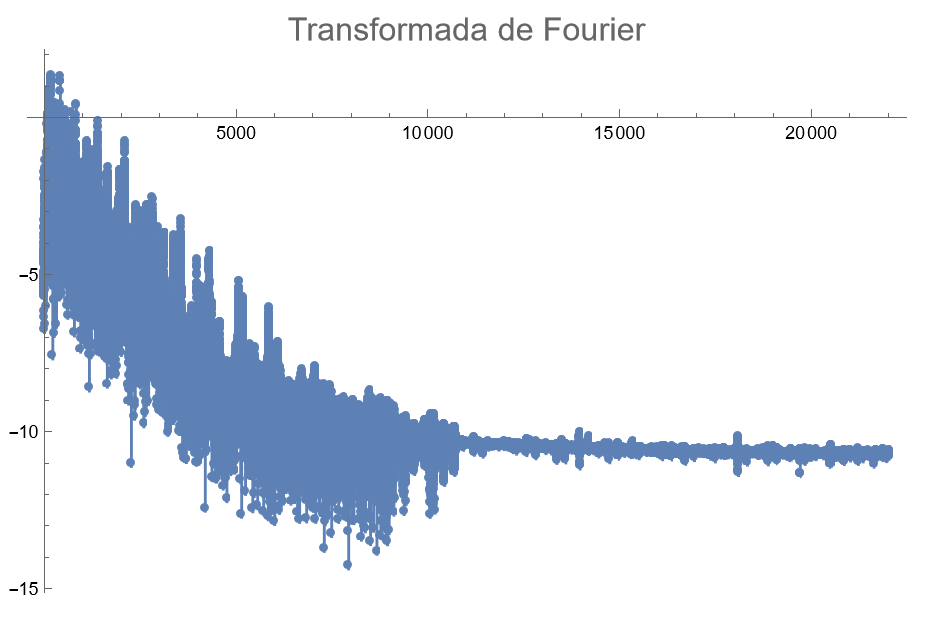
\includegraphics[width=\linewidth]{imgs/Cancion4/transformada.png}
    \captionof{figure}{Logaritmo de la transformada de Fourier de la canción 4}
    \label{fig:04a}
  \end{minipage}
  \begin{minipage}{0.07\textwidth}\end{minipage}
  \begin{minipage}{.47\linewidth}
    \centering
    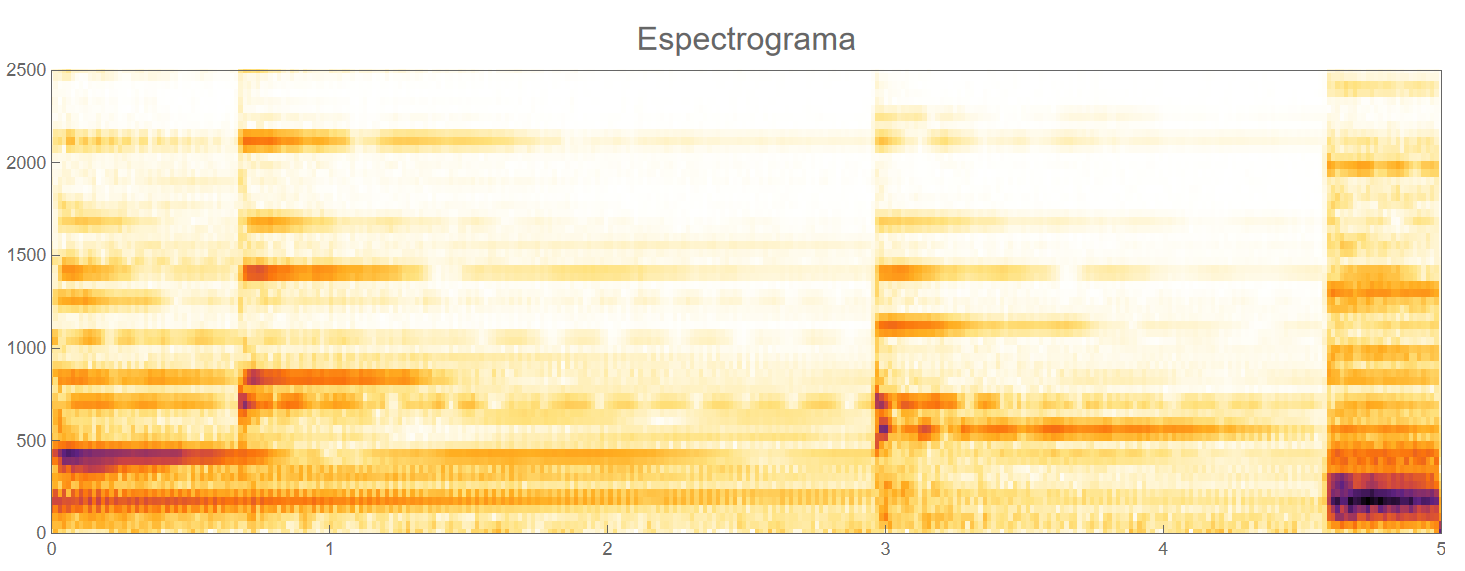
\includegraphics[width=\linewidth]{imgs/Cancion4/espectrograma.png}
    \caption{Espectrograma de la canción 4}
    \label{fig:04i}
  \end{minipage}
\end{figure}
\begin{figure}[H]
  \centering
  \begin{minipage}{.3\textwidth}
    \centering
    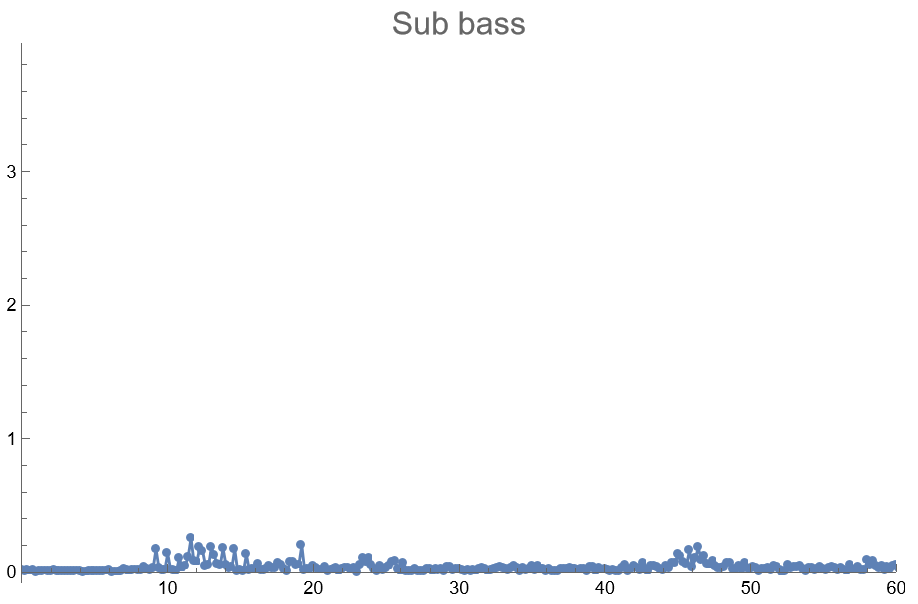
\includegraphics[width=.9\linewidth]{imgs/Cancion4/subbass.png}
  \end{minipage}
  \begin{minipage}{0.03\textwidth}\end{minipage}
  \begin{minipage}{.3\textwidth}
    \centering
    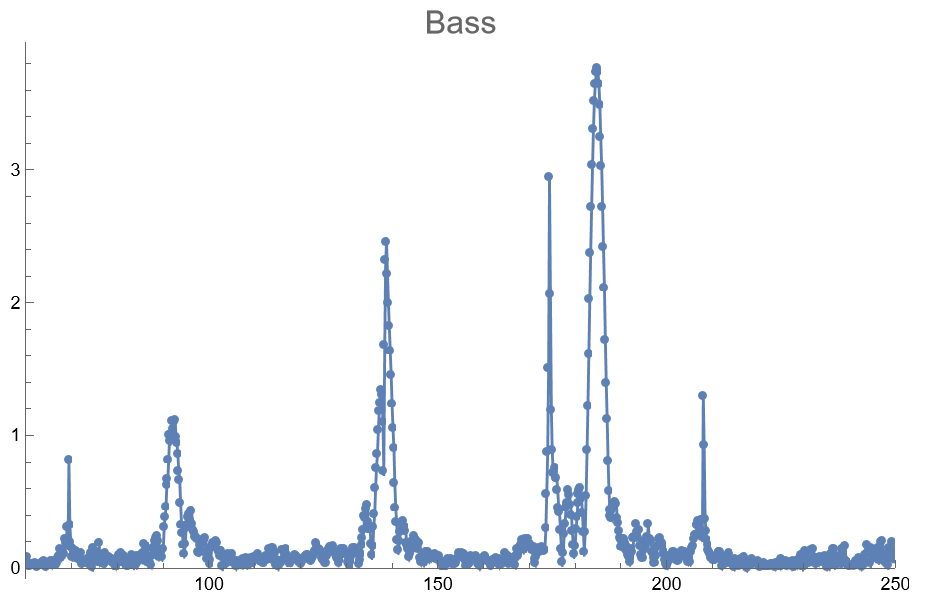
\includegraphics[width=.9\linewidth]{imgs/Cancion4/bass.png}
  \end{minipage} \medskip \\
  \begin{minipage}{.3\textwidth}
    \centering
    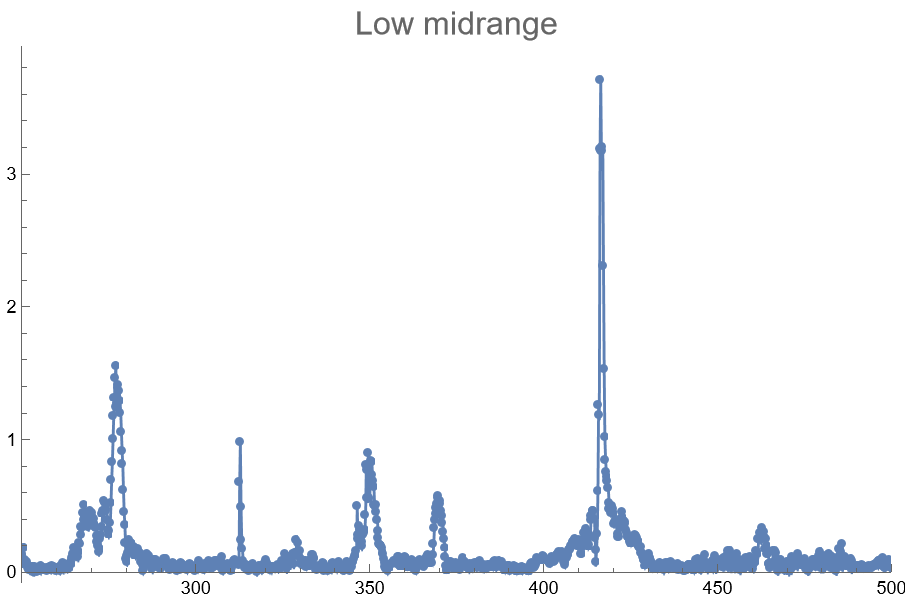
\includegraphics[width=.9\linewidth]{imgs/Cancion4/lowmid.png}
  \end{minipage}
  \begin{minipage}{0.03\textwidth}\end{minipage}
  \begin{minipage}{.3\textwidth}
    \centering
    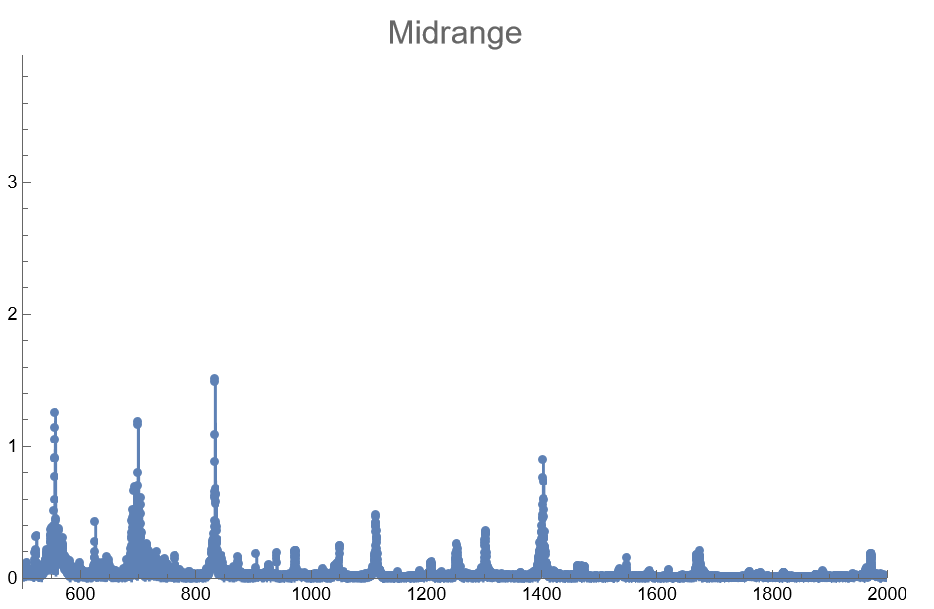
\includegraphics[width=.9\linewidth]{imgs/Cancion4/mid.png}
  \end{minipage}
  \begin{minipage}{0.03\textwidth}\end{minipage}
  \begin{minipage}{.3\textwidth}
    \centering
    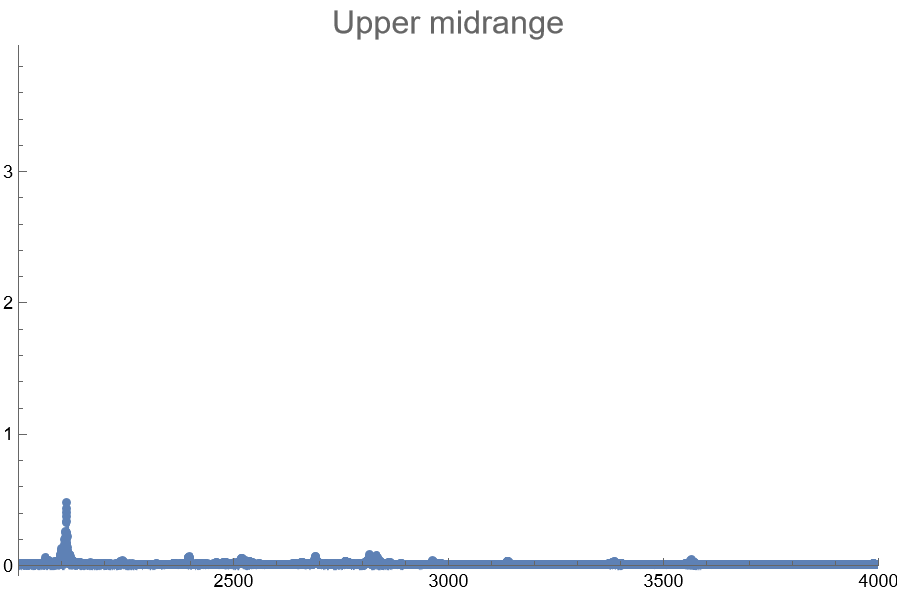
\includegraphics[width=.9\linewidth]{imgs/Cancion4/upmid.png}
  \end{minipage} \medskip \\
  \begin{minipage}{.3\textwidth}
    \centering
    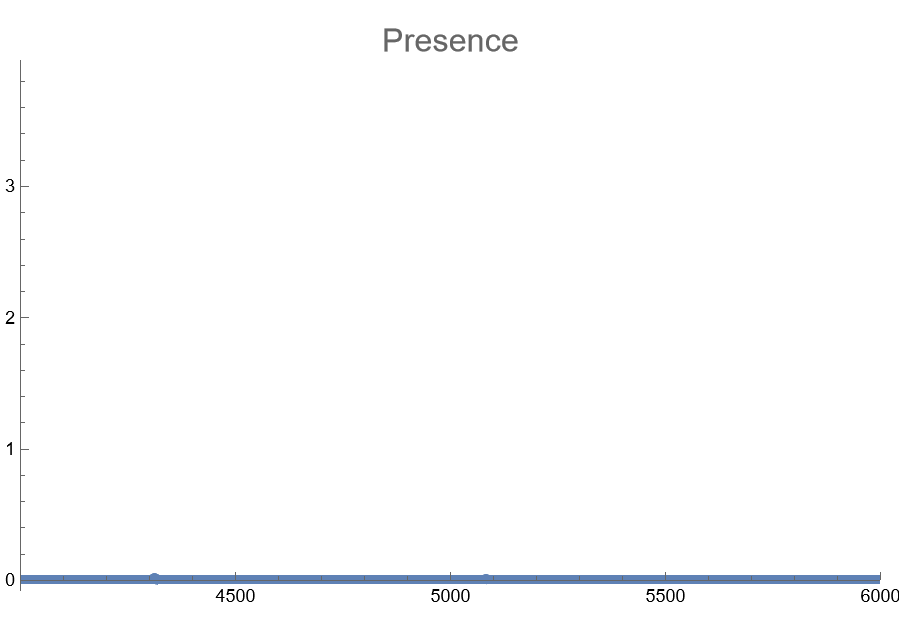
\includegraphics[width=.9\linewidth]{imgs/Cancion4/presence.png}
  \end{minipage}
  \begin{minipage}{0.03\textwidth}\end{minipage}
  \begin{minipage}{.3\textwidth}
    \centering
    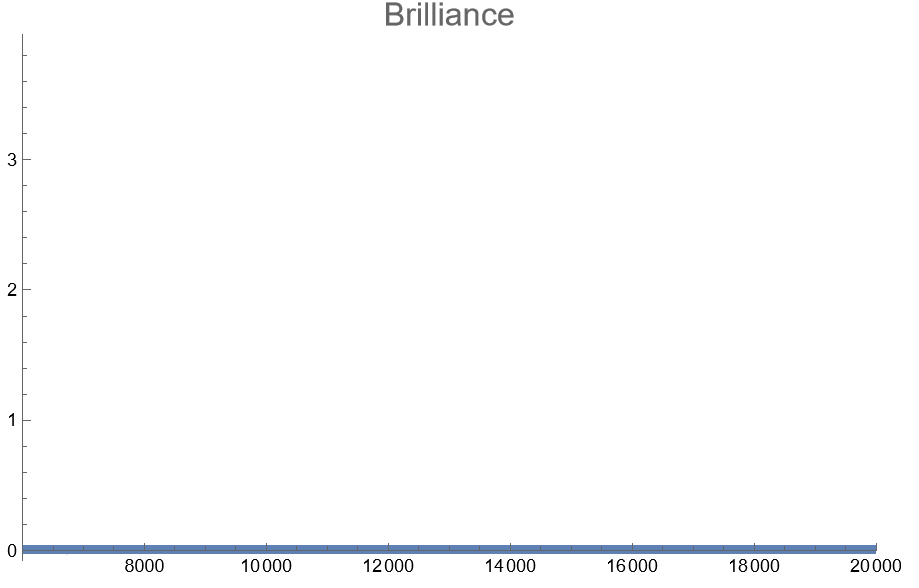
\includegraphics[width=.9\linewidth]{imgs/Cancion4/brilliance.png}
  \end{minipage}
  \caption{Espectro de frecuencias de la canción 4}
  \label{fig:esp04}
\end{figure}

\textbf{Clasificación}: Instrumental

\textbf{Justificación}: El espectro de frecuencias de esta canción no
muestra subbass, por lo que la clasificamos como instrumental. Igualmente,
el espectrograma tiene sonidos que se ven armónicos, así como en la música
instrumental.

\newpage

\textbf{\large{Canción 5}}

\begin{figure}[H]
  \centering
  \begin{minipage}{.4\linewidth}
    \centering
    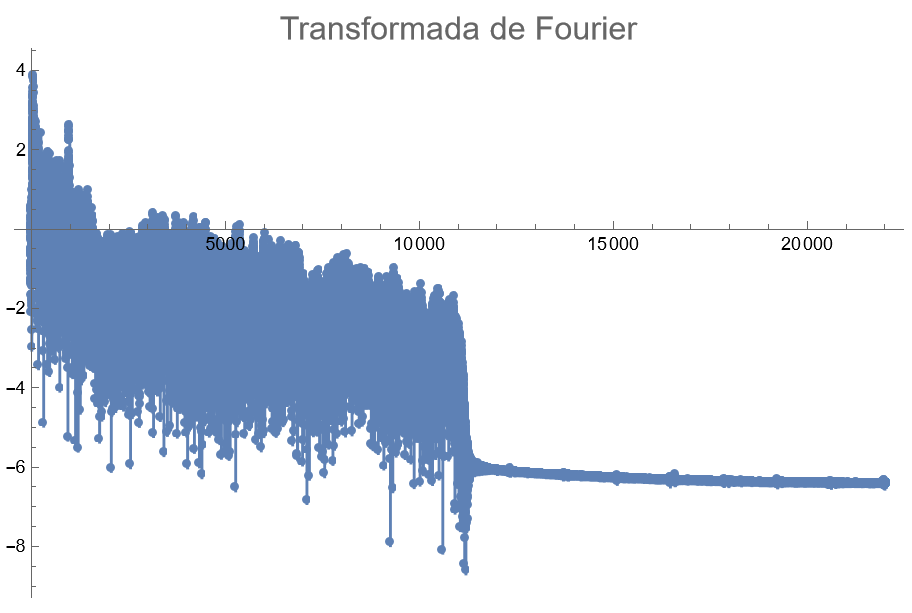
\includegraphics[width=\linewidth]{imgs/Cancion5/transformada.png}
    \captionof{figure}{Logaritmo de la transformada de Fourier de la canción 5}
    \label{fig:05a}
  \end{minipage}
  \begin{minipage}{0.07\textwidth}\end{minipage}
  \begin{minipage}{.47\linewidth}
    \centering
    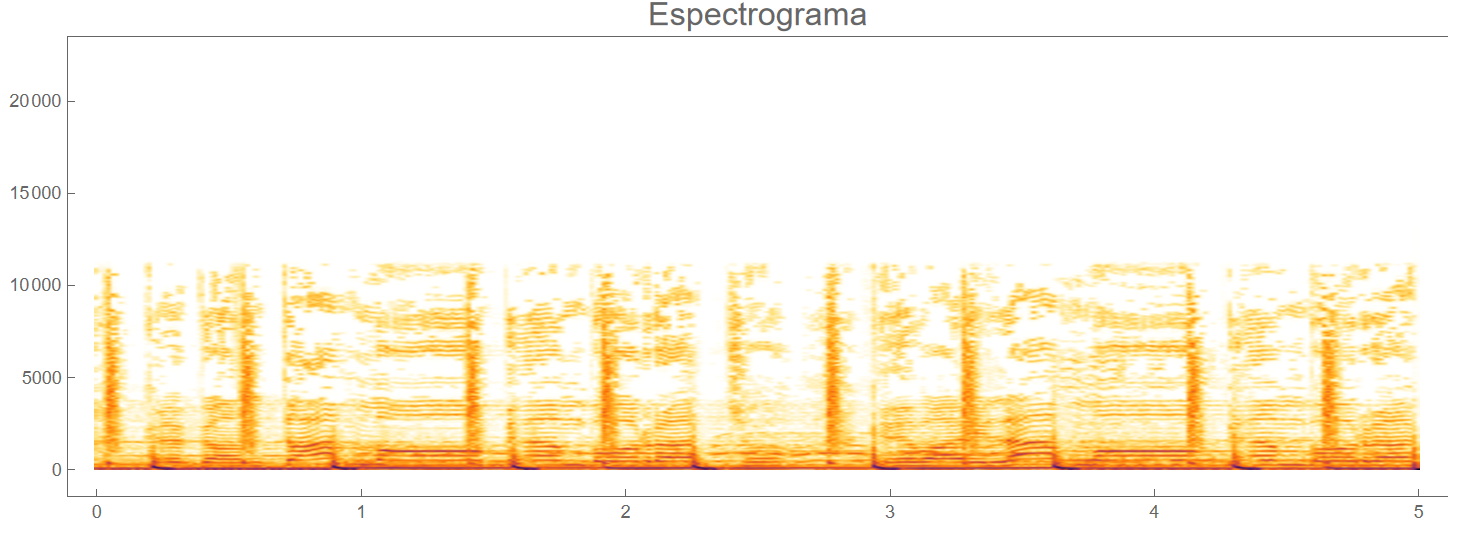
\includegraphics[width=\linewidth]{imgs/Cancion5/espectrograma.png}
    \caption{Espectrograma de la canción 5}
    \label{fig:05i}
  \end{minipage}
\end{figure}
\begin{figure}[H]
  \centering
  \begin{minipage}{.3\textwidth}
    \centering
    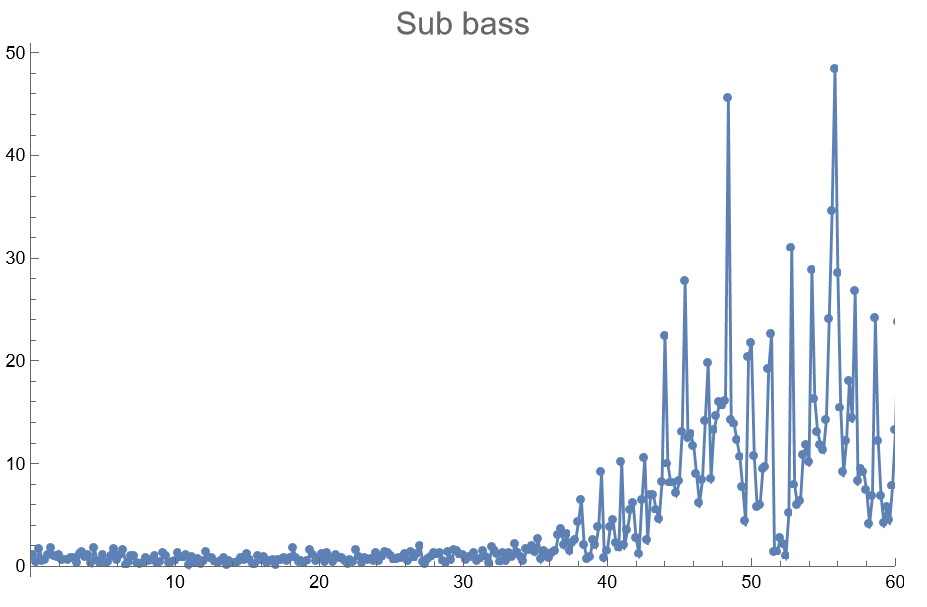
\includegraphics[width=.9\linewidth]{imgs/Cancion5/subbass.png}
  \end{minipage}
  \begin{minipage}{0.03\textwidth}\end{minipage}
  \begin{minipage}{.3\textwidth}
    \centering
    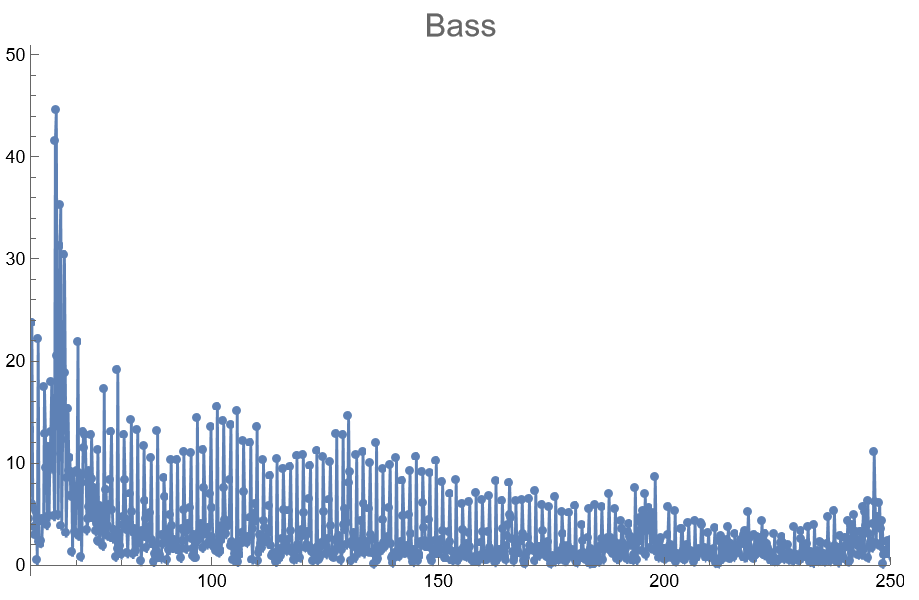
\includegraphics[width=.9\linewidth]{imgs/Cancion5/bass.png}
  \end{minipage} \medskip \\
  \begin{minipage}{.3\textwidth}
    \centering
    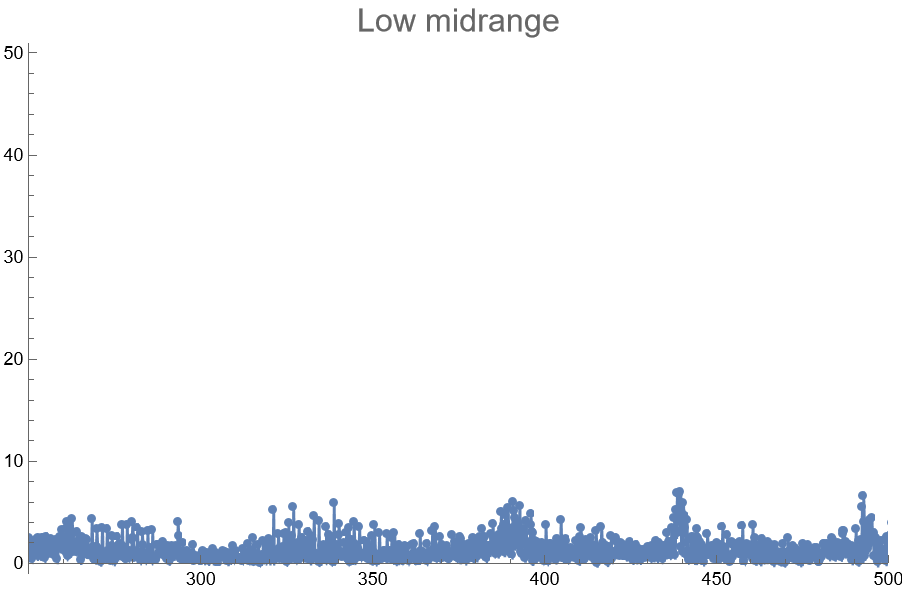
\includegraphics[width=.9\linewidth]{imgs/Cancion5/lowmid.png}
  \end{minipage}
  \begin{minipage}{0.03\textwidth}\end{minipage}
  \begin{minipage}{.3\textwidth}
    \centering
    \includegraphics[width=.9\linewidth]{imgs/Cancion5/mid.png}
  \end{minipage}
  \begin{minipage}{0.03\textwidth}\end{minipage}
  \begin{minipage}{.3\textwidth}
    \centering
    \includegraphics[width=.9\linewidth]{imgs/Cancion5/upmid.png}
  \end{minipage} \medskip \\
  \begin{minipage}{.3\textwidth}
    \centering
    \includegraphics[width=.9\linewidth]{imgs/Cancion5/presence.png}
  \end{minipage}
  \begin{minipage}{0.03\textwidth}\end{minipage}
  \begin{minipage}{.3\textwidth}
    \centering
    \includegraphics[width=.9\linewidth]{imgs/Cancion5/brilliance.png}
  \end{minipage}
  \caption{Espectro de frecuencias de la canción 5}
  \label{fig:esp05}
\end{figure}

\textbf{Clasificación}: Reggaetón

\textbf{Justificación}: En el espectro de frecuencias, se observa
que la canción presenta mucho subbass y bass, indicando que es reggaetón,
y el espectrograma nos lo confirma, al no verse un patrón armónico
tan marcado como en la música instrumental.

\newpage

\textbf{\large{Canción 6}}

\begin{figure}[H]
  \centering
  \begin{minipage}{.4\linewidth}
    \centering
    \includegraphics[width=\linewidth]{imgs/Cancion6/transformada.png}
    \captionof{figure}{Logaritmo de la transformada de Fourier de la canción 6}
    \label{fig:06a}
  \end{minipage}
  \begin{minipage}{0.07\textwidth}\end{minipage}
  \begin{minipage}{.47\linewidth}
    \centering
    \includegraphics[width=\linewidth]{imgs/Cancion6/espectrograma.png}
    \caption{Espectrograma de la canción 6}
    \label{fig:06i}
  \end{minipage}
\end{figure}
\begin{figure}[H]
  \centering
  \begin{minipage}{.3\textwidth}
    \centering
    \includegraphics[width=.9\linewidth]{imgs/Cancion6/subbass.png}
  \end{minipage}
  \begin{minipage}{0.03\textwidth}\end{minipage}
  \begin{minipage}{.3\textwidth}
    \centering
    \includegraphics[width=.9\linewidth]{imgs/Cancion6/bass.png}
  \end{minipage} \medskip \\
  \begin{minipage}{.3\textwidth}
    \centering
    \includegraphics[width=.9\linewidth]{imgs/Cancion6/lowmid.png}
  \end{minipage}
  \begin{minipage}{0.03\textwidth}\end{minipage}
  \begin{minipage}{.3\textwidth}
    \centering
    \includegraphics[width=.9\linewidth]{imgs/Cancion6/mid.png}
  \end{minipage}
  \begin{minipage}{0.03\textwidth}\end{minipage}
  \begin{minipage}{.3\textwidth}
    \centering
    \includegraphics[width=.9\linewidth]{imgs/Cancion6/upmid.png}
  \end{minipage} \medskip \\
  \begin{minipage}{.3\textwidth}
    \centering
    \includegraphics[width=.9\linewidth]{imgs/Cancion6/presence.png}
  \end{minipage}
  \begin{minipage}{0.03\textwidth}\end{minipage}
  \begin{minipage}{.3\textwidth}
    \centering
    \includegraphics[width=.9\linewidth]{imgs/Cancion6/brilliance.png}
  \end{minipage}
  \caption{Espectro de frecuencias de la canción 6}
  \label{fig:esp06}
\end{figure}

\textbf{Clasificación}: Reggaetón

\textbf{Justificación}: Nuevamente hay una gran predominancia en las frecuencias
que se encuentran en el subbass y el bass de la canción, significando así que
la canción es de reggaetón. Asimismo, el espectrograma se asemeja a las demás canciones
clasificadas como reggaetón, debido a su falta de sonidos armónicos preponderantes.


\newpage

\textbf{\large{Canción 7}}

\begin{figure}[H]
  \centering
  \begin{minipage}{.4\linewidth}
    \centering
    \includegraphics[width=\linewidth]{imgs/Cancion7/transformada.png}
    \captionof{figure}{Logaritmo de la transformada de Fourier de la canción 7}
    \label{fig:07a}
  \end{minipage}
  \begin{minipage}{0.07\textwidth}\end{minipage}
  \begin{minipage}{.47\linewidth}
    \centering
    \includegraphics[width=\linewidth]{imgs/Cancion7/espectrograma.png}
    \caption{Espectrograma de la canción 7}
    \label{fig:07i}
  \end{minipage}
\end{figure}
\begin{figure}[H]
  \centering
  \begin{minipage}{.3\textwidth}
    \centering
    \includegraphics[width=.9\linewidth]{imgs/Cancion7/subbass.png}
  \end{minipage}
  \begin{minipage}{0.03\textwidth}\end{minipage}
  \begin{minipage}{.3\textwidth}
    \centering
    \includegraphics[width=.9\linewidth]{imgs/Cancion7/bass.png}
  \end{minipage} \medskip \\
  \begin{minipage}{.3\textwidth}
    \centering
    \includegraphics[width=.9\linewidth]{imgs/Cancion7/lowmid.png}
  \end{minipage}
  \begin{minipage}{0.03\textwidth}\end{minipage}
  \begin{minipage}{.3\textwidth}
    \centering
    \includegraphics[width=.9\linewidth]{imgs/Cancion7/mid.png}
  \end{minipage}
  \begin{minipage}{0.03\textwidth}\end{minipage}
  \begin{minipage}{.3\textwidth}
    \centering
    \includegraphics[width=.9\linewidth]{imgs/Cancion7/upmid.png}
  \end{minipage} \medskip \\
  \begin{minipage}{.3\textwidth}
    \centering
    \includegraphics[width=.9\linewidth]{imgs/Cancion7/presence.png}
  \end{minipage}
  \begin{minipage}{0.03\textwidth}\end{minipage}
  \begin{minipage}{.3\textwidth}
    \centering
    \includegraphics[width=.9\linewidth]{imgs/Cancion7/brilliance.png}
  \end{minipage}
  \caption{Espectro de frecuencias de la canción 7}
  \label{fig:esp07}
\end{figure}

\textbf{Clasificación}: Instrumental

\textbf{Justificación}: La canción no presenta una gran predominancia
de frecuencias dentro del subbass, y su espectrograma muestra muchos sonidos
armónicos, por lo que la clasificamos como instrumental.

\newpage

\textbf{\large{Canción 8}}

\begin{figure}[H]
  \centering
  \begin{minipage}{.4\linewidth}
    \centering
    \includegraphics[width=\linewidth]{imgs/Cancion8/transformada.png}
    \captionof{figure}{Logaritmo de la transformada de Fourier de la canción 8}
    \label{fig:08a}
  \end{minipage}
  \begin{minipage}{0.07\textwidth}\end{minipage}
  \begin{minipage}{.47\linewidth}
    \centering
    \includegraphics[width=\linewidth]{imgs/Cancion8/espectrograma.png}
    \caption{Espectrograma de la canción 8}
    \label{fig:08i}
  \end{minipage}
\end{figure}
\begin{figure}[H]
  \centering
  \begin{minipage}{.3\textwidth}
    \centering
    \includegraphics[width=.9\linewidth]{imgs/Cancion8/subbass.png}
  \end{minipage}
  \begin{minipage}{0.03\textwidth}\end{minipage}
  \begin{minipage}{.3\textwidth}
    \centering
    \includegraphics[width=.9\linewidth]{imgs/Cancion8/bass.png}
  \end{minipage} \medskip \\
  \begin{minipage}{.3\textwidth}
    \centering
    \includegraphics[width=.9\linewidth]{imgs/Cancion8/lowmid.png}
  \end{minipage}
  \begin{minipage}{0.03\textwidth}\end{minipage}
  \begin{minipage}{.3\textwidth}
    \centering
    \includegraphics[width=.9\linewidth]{imgs/Cancion8/mid.png}
  \end{minipage}
  \begin{minipage}{0.03\textwidth}\end{minipage}
  \begin{minipage}{.3\textwidth}
    \centering
    \includegraphics[width=.9\linewidth]{imgs/Cancion8/upmid.png}
  \end{minipage} \medskip \\
  \begin{minipage}{.3\textwidth}
    \centering
    \includegraphics[width=.9\linewidth]{imgs/Cancion8/presence.png}
  \end{minipage}
  \begin{minipage}{0.03\textwidth}\end{minipage}
  \begin{minipage}{.3\textwidth}
    \centering
    \includegraphics[width=.9\linewidth]{imgs/Cancion8/brilliance.png}
  \end{minipage}
  \caption{Espectro de frecuencias de la canción 8}
  \label{fig:esp08}
\end{figure}

\textbf{Clasificación}: Instrumental

\textbf{Justificación}: Nuevamente, observamos poco subbass en el espectro de
frecuencias, y sonidos armónicos en el espectrograma, que significan una canción
instrumental.

\newpage

\textbf{\large{Canción 9}}

\begin{figure}[H]
  \centering
  \begin{minipage}{.4\linewidth}
    \centering
    \includegraphics[width=\linewidth]{imgs/Cancion9/transformada.png}
    \captionof{figure}{Logaritmo de la transformada de Fourier de la canción 9}
    \label{fig:09a}
  \end{minipage}
  \begin{minipage}{0.07\textwidth}\end{minipage}
  \begin{minipage}{.47\linewidth}
    \centering
    \includegraphics[width=\linewidth]{imgs/Cancion9/espectrograma.png}
    \caption{Espectrograma de la canción 9}
    \label{fig:09i}
  \end{minipage}
\end{figure}
\begin{figure}[H]
  \centering
  \begin{minipage}{.3\textwidth}
    \centering
    \includegraphics[width=.9\linewidth]{imgs/Cancion9/subbass.png}
  \end{minipage}
  \begin{minipage}{0.03\textwidth}\end{minipage}
  \begin{minipage}{.3\textwidth}
    \centering
    \includegraphics[width=.9\linewidth]{imgs/Cancion9/bass.png}
  \end{minipage} \medskip \\
  \begin{minipage}{.3\textwidth}
    \centering
    \includegraphics[width=.9\linewidth]{imgs/Cancion9/lowmid.png}
  \end{minipage}
  \begin{minipage}{0.03\textwidth}\end{minipage}
  \begin{minipage}{.3\textwidth}
    \centering
    \includegraphics[width=.9\linewidth]{imgs/Cancion9/mid.png}
  \end{minipage}
  \begin{minipage}{0.03\textwidth}\end{minipage}
  \begin{minipage}{.3\textwidth}
    \centering
    \includegraphics[width=.9\linewidth]{imgs/Cancion9/upmid.png}
  \end{minipage} \medskip \\
  \begin{minipage}{.3\textwidth}
    \centering
    \includegraphics[width=.9\linewidth]{imgs/Cancion9/presence.png}
  \end{minipage}
  \begin{minipage}{0.03\textwidth}\end{minipage}
  \begin{minipage}{.3\textwidth}
    \centering
    \includegraphics[width=.9\linewidth]{imgs/Cancion9/brilliance.png}
  \end{minipage}
  \caption{Espectro de frecuencias de la canción 9}
  \label{fig:esp09}
\end{figure}

\textbf{Clasificación}: Reggaetón

\textbf{Justificación}: Esta canción no parece presentar un subbass tan dominante,
aunque no se observa tan insignificante como en otras canciones instrumentales.
Observando más a detalle, las magnitudes de las frecuencias en el subbass de
otras canciones instrumentales han sido menores a 1, y estas llegan a más de 7.
Asimismo, observando el espectrograma de esta canción, no se presentan sonidos
armónicos. Con todo ello, concluimos que esta canción es de reggaetón.

\newpage

\textbf{\large{Canción 10}}

\begin{figure}[H]
  \centering
  \begin{minipage}{.4\linewidth}
    \centering
    \includegraphics[width=\linewidth]{imgs/Cancion10/transformada.png}
    \captionof{figure}{Logaritmo de la transformada de Fourier de la canción 10}
    \label{fig:010a}
  \end{minipage}
  \begin{minipage}{0.07\textwidth}\end{minipage}
  \begin{minipage}{.47\linewidth}
    \centering
    \includegraphics[width=\linewidth]{imgs/Cancion10/espectrograma.png}
    \caption{Espectrograma de la canción 10}
    \label{fig:010i}
  \end{minipage}
\end{figure}
\begin{figure}[H]
  \centering
  \begin{minipage}{.3\textwidth}
    \centering
    \includegraphics[width=.9\linewidth]{imgs/Cancion10/subbass.png}
  \end{minipage}
  \begin{minipage}{0.03\textwidth}\end{minipage}
  \begin{minipage}{.3\textwidth}
    \centering
    \includegraphics[width=.9\linewidth]{imgs/Cancion10/bass.png}
  \end{minipage} \medskip \\
  \begin{minipage}{.3\textwidth}
    \centering
    \includegraphics[width=.9\linewidth]{imgs/Cancion10/lowmid.png}
  \end{minipage}
  \begin{minipage}{0.03\textwidth}\end{minipage}
  \begin{minipage}{.3\textwidth}
    \centering
    \includegraphics[width=.9\linewidth]{imgs/Cancion10/mid.png}
  \end{minipage}
  \begin{minipage}{0.03\textwidth}\end{minipage}
  \begin{minipage}{.3\textwidth}
    \centering
    \includegraphics[width=.9\linewidth]{imgs/Cancion10/upmid.png}
  \end{minipage} \medskip \\
  \begin{minipage}{.3\textwidth}
    \centering
    \includegraphics[width=.9\linewidth]{imgs/Cancion10/presence.png}
  \end{minipage}
  \begin{minipage}{0.03\textwidth}\end{minipage}
  \begin{minipage}{.3\textwidth}
    \centering
    \includegraphics[width=.9\linewidth]{imgs/Cancion10/brilliance.png}
  \end{minipage}
  \caption{Espectro de frecuencias de la canción 10}
  \label{fig:esp010}
\end{figure}

\textbf{Clasificación}: Instrumental

\textbf{Justificación}: El espectrograma muestra sonidos armónicos, y el
espectro de frecuencias no presenta magnitudes altas de frecuencias, por lo que
clasificamos esta canción como instrumental.

\newpage

\section{Conclusiones}

En conclusión, esta actividad ha mostrado cómo el análisis espectral, mediante la Transformada de Fourier, 
puede ser utilizado eficazmente para clasificar géneros musicales como el reggaetón y la música instrumental. 
Al analizar el espectro de frecuencias y los espectrogramas, se observó que el reggaetón tiene una predominancia 
de frecuencias bajas, especialmente en los rangos de subbass y bass, lo que le da una textura más compleja y saturada. 
Por otro lado, la música instrumental mostró frecuencias más armónicas y definidas, con una estructura más ordenada en el espectrograma.

Este enfoque resalta cómo las matemáticas y la física, a través de herramientas como la Transformada de Fourier, 
pueden ser aplicadas para entender y clasificar diferentes tipos de sonidos. Además, demuestra el potencial de este 
tipo de análisis no solo en la música, sino en el procesamiento de señales en general, con aplicaciones en áreas como 
el reconocimiento de audio y la mejora de la calidad sonora. En resumen, la metodología utilizada abre nuevas 
posibilidades para el análisis musical y el desarrollo de tecnologías en el campo del procesamiento de señales.



\begin{thebibliography}{9}
  \bibitem{university-physics}
  H. D. Young and Roger A. Freedman, \emph{University Physics with Modern Physics}, 
  Addison-Wesley, San Francisco, 2012.
  \bibitem{frequencies-wave-sound-pso}
  Al Hwaitat et Al, Journal of Experimental \&\ Theoretical Artificial Intelligence,
  2022, 34, 749-780.
  \bibitem{orchestra-frecuency}
  N. Lenssen, \emph{PhD Thesis: Applications of Fourier Analysis to Audio Signal Processing: An Investigation of Chord Detection Algorithms
  }, Claremont University, 2013.
  \bibitem{octave-definition}
  Britannica, https://www.britannica.com/art/octave-music, (accesado 28 Octubre 2024).
  \bibitem{Montenegro-2009}
  A. Montenegro, \textit{CORE}, 2009, \url{https://core.ac.uk/download/pdf/6448967.pdf}, (accesado Octubre 28, 2024).
  \bibitem{Bernal-1999}
  J. Bernal, P. Gómez y J. Bobadilla, \textit{Estudios de fonética experimental}, 1999, \textbf{10}, 75-105.
  \bibitem{OGorman-2023}
  L. O'Gorman, \textit{DIBS Methods Meetings}, 2023, \url{https://dibsmethodsmeetings.github.io/fourier-transforms/}.
  \bibitem{Costa-2011}
  Y. M. G. Costa, L. S. Oliveira, A. L. Koerich y F. Gouyon, \textit{IEEE}, 2011,
  \textbf{18}, 1-4.
  \bibitem{Colomer-01}
  Luis Colomer Blasco, Capítulo 10. Figura 10. Espectrograma serie armónica,
  \url{https://www.youtube.com/watch?v=RzitKHMUoeg}, (accesado Octubre 28, 2024).
  \bibitem{Colomer-02}
  Luis Colomer Blasco, Capítulo 10. Figura 11. Espectrograma de envolventes de amplitud,
  \url{https://www.youtube.com/watch?v=idEvt5HuQTc}, (accesado Octubre 28, 2024).
  % \bibitem{Colomer-03}
  % Luis Colomer Blasco, Capítulo 10. Figura 12. Espectrograma de envolventes de frecuencia,
  % \url{https://www.youtube.com/watch?v=RV2Ev9zhe5E}, (accesado Octubre 28, 2024)
  \bibitem{Colomer-04}
  Luis Colomer Blasco, Capítulo 10. Figura 13. Espectrograma de ruido blanco y sonido simple,
  \url{https://www.youtube.com/watch?v=ZoffBnGMctI}, (accesado Octubre 28, 2024).
  \bibitem{Colomer-05}
  Luis Colomer Blasco, Capítulo 10. Figura 14. Espectrograma de tráfico con lluvia y locutora de radio,
  \url{https://www.youtube.com/watch?v=XUvLZQctg7I}, (accesado Octubre 28, 2024).
  \bibitem{Gleeson-2024}
  Headphonesty, \url{https://www.headphonesty.com/2020/02/audio-frequency-spectrum-explained/},
  (accesado Noviembre 04, 2024).
  \bibitem{fink-2018}
  R. Fink, M. Latour y Z. Wallmark, \textit{The Relentless Pursuit of Tone: Timbre in Popular Music},
  Oxford University Press, 2018.
  \bibitem{Garcia-2016}
  L. M. Garcia, \textit{Sound Studies: An Interdisciplinary Journal}, 2016, \textbf{1}, 59-76.
\end{thebibliography}
\end{document}